\documentclass{article}
\usepackage[table]{xcolor}
\usepackage[T1]{fontenc}
\usepackage{tgschola}
\usepackage[a4paper, total={6in, 8in}, margin=2cm]{geometry}
\usepackage{lipsum}
\usepackage{fancyhdr}
\usepackage{lastpage}
\setlength{\headheight}{48.2pt}
\usepackage{boxedminipage}
\usepackage{graphicx}
\usepackage{tikz}
\usetikzlibrary{shapes.geometric}
\usepackage{wrapfig}
\usepackage{float}
\usepackage{subfig}
\usepackage{circuitikz}
\usetikzlibrary{arrows}
\usepackage[T1]{fontenc}
\usepackage{tgbonum}
\usepackage[most]{tcolorbox}
\usepackage{textgreek}
\usepackage{graphicx}
\graphicspath{ {./} }
\usepackage[T1]{fontenc}
\usepackage{multicol}
\usepackage{siunitx}
\sisetup{output-decimal-marker = {,}} %para que use coma en vez de punto
\usepackage[usestackEOL]{stackengine}
\graphicspath{ {./imagenes/} }
\pagestyle{fancy}
\usepackage{enumitem}
\usepackage[most]{tcolorbox}
\usepackage[option ]{askmaps}
\usepackage{circuitikz}
\usepackage{float}
\usepackage{adjustbox}
\usepackage{amsmath}
\usepackage{array}
\usepackage{multirow}
\usepackage{geometry}
\usepackage{booktabs}
\usepackage{tikz-timing}
\usepackage{url}
\usepackage{fancyvrb}
\usepackage{fvextra}
\usepackage[implicit=false]{hyperref}

\definecolor{headergray}{RGB}{220,220,220}
\usepackage{geometry}
\usepackage{changepage}
\usepackage{listings}
\lstset{
	basicstyle=\small\ttfamily,
	columns=flexible,
	breaklines=true
}
\usepackage{skull}
\usepackage{makecell}

%%Modificar los siguientes valores segun la materia/tp
\newcommand{\Titulo}{Trabajo Práctico 1.2-1.3}
\newcommand{\Subtitulo}{Semiconductores y tecnología }
\newcommand{\SubtituloDos}{de circuitos integrados}
\newcommand{\Version}{Versión 261C.01}
\newcommand{\Carrera}{INGENIERÍA EN INFORMÁTICA}
\newcommand{\Asignatura}{3631 - Fundamentos de sistemas embebidos}
\newcommand{\Tema}{Semiconductores y tecnología de circuitos integrados}
\newcommand{\Unidad}{1.2 - 1.3}
\newcommand{\Objetivo}{Comprender los conceptos básicos de semiconductores y las características de las señales digitales en circuitos integrados}
\newcommand{\TiempoResolucion}{1 semana}
\newcommand{\Metodologia}{Ejercicios verificados en simuladores}
\newcommand{\Entrega}{No obligatoria}


\fancyhead[L]{\framebox(128,64){\includegraphics[scale=0.18]{diit}}}
\fancyhead[C]{\framebox(224,64){\Longstack{\textbf{\Titulo}\\\textbf{\Subtitulo}\\\textbf{\SubtituloDos}\\Pág. \thepage\ de \pageref{LastPage}}}}
\fancyhead[R]{\framebox(128,64){\includegraphics[scale=0.055]{logo}}}
\renewcommand{\headrulewidth}{0.0pt}
\renewcommand{\footrulewidth}{0pt}



\begin{document}
	
		\centering\LARGE{\textbf{\Version}}
	\large
	\\
	\begin{center}
		\begin{tabular}{|p{16cm}|} % 'l' for left-aligned, 'p' for paragraph with specified width
			
			\hline
			\rule{0pt}{15pt}
			\textbf{Carrera: \Carrera} \\
			\hline
			\rule{0pt}{15pt}
			\textbf{Asignatura:}  \Asignatura \\
			\hline
			\rule{0pt}{15pt}
			\textbf{Tema:}  \Tema \\
			\hline
			\rule{0pt}{15pt}
			\textbf{Unidad:}  \Unidad \\
			\hline
			\rule{0pt}{15pt}
			\textbf{Objetivo:} \Objetivo \\
			\hline
			\rule{0pt}{15pt}
			\textbf{Competencias a desarrollar:} 
			\begin{itemize}
				\item Concepción, diseño y desarrollo de proyectos de ingeniería en informática.
				\item Gestión, planificación, ejecución y control de proyectos de ingeniería en informática.
				\item Utilización de técnicas y herramientas de aplicación en la ingeniería en informática.
				\item Generación de desarrollos tecnológicos y/o innovaciones tecnológicas.
				\item Desarrollo de una actitud profesional emprendedora.
				\item Aprendizaje continuo
				\item Actuación profesional ética y responsable.
				\item Comunicación efectiva.
				\item Desempeño en equipos de trabajo.
				\item Identificación, formulación y resolución de problemas de ingeniería en informática
			\end{itemize} \\
			\hline
			\rule{0pt}{15pt}
			\textbf{Descripción de la actividad:} 
			\begin{enumerate}
				\item  Tiempo estimado de resolución: \TiempoResolucion
				\item Metodología: \Metodologia
				\item Forma de entrega: \Entrega
				\item Metodología de corrección y feedback al alumno: Presencial y por Miel.
			\end{enumerate} \\
			\hline
		\end{tabular}
	\end{center}
	
	\clearpage
	
			%% Hacer que las tablas tengan un poco de padding
	\def\arraystretch{1.2}
	
	\section*{B- Semiconductores}
	\begin{adjustwidth}{-25pt}{-20pt}
		\begin{tcolorbox}[enhanced,attach boxed title to top center={yshift=-3mm,yshifttext=-1mm},
			colback=black!5!white,colframe=white!75!black,colbacktitle=red!80!black,
			title= Diodo Ideal vs Diodo Real , fonttitle=\bfseries,
			boxed title style={size=small,colframe=white,colback=black} ]
			Dado que cada diodo tiene una curva que describe su funcionamiento, en cada ejercicio se indica si se utiliza un diodo real o un diodo ideal. Los ejercicios que se refieren al diodo ideal de 2V utilizan el siguiente subcircuito visto en la teoría. A continuación dejamos el texto del subcircuito para el simulador Falstad, que puede importarse en  File > Import From Text , y luego una vez importado File > Create Subcircuit para poder incluirlo en Draw > Subcircuit.
			\begin{lstlisting}
$ 65 0.000005 10.20027730826997 50 5 50 5e-11
207 240 112 240 80 4 Anodo
207 240 144 240 176 4 Catodo
a 320 128 384 128 9 15 -15 1000000 0.9999699751152668 0.999989974715225 100000
178 432 32 512 32 6 1 0.2 1.9990001103309396e-10 0.05 1000000 0.02 20 0.015 0.005 0
v 240 144 208 144 0 0 40 2 0 0 0.5
R 432 80 400 80 0 0 40 1.999 0 0 0.5
401 432 112 512 112 1 8\s15\s-15\s1000000\s1.9999599958175907\s1.999\s100000 2\s20\s10000000000\s2.5 1\s0
r 320 176 384 176 0 10000000
r 320 112 240 112 0 10000000
r 320 144 240 144 0 10000000
w 320 176 320 144 0
w 384 176 384 128 0
r 320 80 384 80 0 10000000
w 320 80 320 112 0
g 384 80 384 96 0 0
w 432 64 432 80 0
w 432 96 432 80 0
w 512 112 512 64 0
w 240 112 208 112 0
w 208 112 208 32 0
w 432 128 384 128 0
w 208 32 432 32 0
w 208 144 208 192 0
w 208 192 528 192 0
w 528 192 528 16 0
w 528 16 512 16 0

				\end{lstlisting}
				\begin{tikzpicture}
					% Paths, nodes and wires:
					\node[squarepole] at (3.25, 7.5){};
					\node[squarepole] at (3.25, 5.5){};
					\node[op amp, yscale=-1] at (7.083, 6.539){};
					\draw (4, 7) to[american resistor] (5.893, 7.029);
					\draw (5.833, 8.039) to[american resistor] (7.833, 8.039);
					\node[ground] at (7.833, 8.039){};
					\node[circ] at (5.833, 7.039){};
					\draw (5.833, 8.039) -| (5.833, 7.039);
					\draw (4, 6) to[american resistor] (5.893, 6.049);
					\node[circ] at (5.833, 6.039){};
					\draw (5.833, 5.039) to[american resistor] (8.333, 5.039);
					\draw (5.833, 5.039) -| (5.833, 6.039);
					\draw (8.333, 6.539) -- (8.333, 5.039);
					\node[circ] at (4, 7){};
					\node[circ] at (4, 6){};
					\node[spdt, yscale=-1] at (9.905, 9.435){};
					\draw (10.5, 9.75) to[battery1] (11.405, 9.75);
					\node[shape=rectangle, minimum width=0.965cm, minimum height=0.715cm](N1) at (3.25, 7.875){} node[anchor=center] at (N1.text){$Anodo$};
					\node[shape=rectangle, minimum width=0.965cm, minimum height=0.715cm](N2) at (3.25, 5.125){} node[anchor=center] at (N2.text){$Catodo$};
					\draw (8.595, 8.25) to[cute inductor] (11.095, 8.25);
					\node[vcc](N3) at (8.655, 8.25){} node[anchor=east] at ([xshift=0.18cm]N3.west){$2V$};
					\node[op amp](N4) at (9.845, 7){} node[anchor=east] at ([xshift=-0.62cm]N4.east){$\geq?$};
					\node[circ] at (8.655, 8.25){};
					\draw (8.655, 7.49) |- (8.595, 8.25);
					\draw (11.095, 7) -| (11.095, 8.25);
					\node[shape=rectangle, draw, line width=1pt, dash pattern={on 4pt off 4pt}, minimum width=1.215cm, minimum height=1.965cm] at (9.875, 9){};
					\node[circ] at (8.333, 6.539){};
					\draw (8.655, 6.51) -| (8.333, 6.539);
					\draw (4, 7) -| (3.25, 7.5);
					\draw (4, 6) |- (3.25, 6) -| (3.25, 5.5);
					\draw (11.405, 9.75) |- (4, 4.5) -| (4, 6);
					\draw (9.31, 9.435) -| (4, 7);
				\end{tikzpicture}
				\\ Recuerde que esto \textbf{NO ES UN DIODO} sino un subcircuito creado para "simular" un diodo ideal ya que el mismo no existe.
		\end{tcolorbox}
	\end{adjustwidth}
	

		\begin{enumerate}[label=\textbf{B.\arabic*},resume]	
		\begin{minipage}{.75\textwidth} 
			\item
			\label{diodobasico}
			Dado el siguiente circuito complete los valores que faltan en la tabla. El diodo $D1$ equivale al diodo ideal de 2V simulado. Considerando que comercialmente se consiguen resistores de $1/8W,1/4W,1/2W,1W,2W,5W$, indique el adecuado. \textit{Nota: Recuerde que este diodo no conduce hasta no esta polarizado en directa con al menos 2V de diferencia de potencial entre ánodo y cátodo, luego se comporta como una llave ideal.}  
		\end{minipage}
		\begin{minipage}{.90\textwidth}
			\begin{tikzpicture}
				% Paths, nodes and wires:
				\node[circ] at (6, 8){};
				\draw (4, 8.5) to[battery1, l_={$V1$}] (4, 7.5);
				\node[plain crossing] at (3.75, 8.36){};
				\draw (6, 8) to[american resistor, l={$R1$}] (6, 10);
				\draw (6, 8) to[empty diode, l_={$D1$}] (6, 6);
				\draw (4, 8.5) -| (4, 10) -- (6, 10);
				\draw (6, 6) -- (4, 6) -| (4, 7.5);
				\node[shape=rectangle, minimum width=0.715cm, minimum height=0.465cm](N1) at (6.375, 8){} node[anchor=center] at (N1.text){$Va$};
				\node[shape=rectangle, minimum width=0.715cm, minimum height=0.465cm](N2) at (3.5, 9.5){} node[anchor=center] at (N2.text){$i1$};
				\draw[-latex] (3.75, 9) -- (3.75, 10);
			\end{tikzpicture}
		\end{minipage}
		\\
		\begin{tabular}{|c|c|c|c|c|c|c|c|}
			\hline
			\rowcolor{headergray}
			${V1 }$& ${R1}$& ${i1}$&$Va$&$V_{R1}$&$P_{R1}$&$D1$&$W_{res}$\\ \hline
			$\SI{5}{\volt}$& $\SI{300}{\ohm}$& $\SI{10}{\milli\ampere}$& $\SI{2}{\volt}$&$\SI{3}{\volt}$&$\SI{30}{\milli\watt}$& $\SI{2}{\volt}$&$1/8W$ \\ \hline
			$\SI{5}{\volt}$&&$\SI{20}{\milli\ampere}$&&&&$\SI{2}{\volt}$ & \\ \hline
			$\SI{12}{\volt}$&&&&$\SI{10}{\volt}$&$\SI{200}{\milli\watt}$&$\SI{2}{\volt}$ & \\ \hline
			& $\SI{21,8}{\kilo\ohm}$&&&$\SI{218}{\volt}$&&$\SI{2}{\volt}$ & \\ \hline
			$\SI{1}{\volt}$&$\SI{2}{\ohm}$&&$\SI{1}{\volt}$&&&$\SI{2}{\volt}$& \\ \hline
			
		\end{tabular}
		\\
		\item Dado el circuito del punto \ref{diodobasico} el diodo $D1$ equivale al 1N4004 (diodo real). Encuentre los valores faltantes en la tabla. \textit{Nota: tenga en cuenta que al ser un diodo real, su tensión de umbral (D1) va a depender de la corriente que circula por el mismo, por ende no desprecie decimales para que los valores calculados se acerquen lo mas posible a la simulación.} \label{b2}
		\\
		\begin{tabular}{|c|c|c|c|c|c|c|c|}
			\hline
			\rowcolor{headergray}
			${V1 }$& ${R1}$& ${i1}$&$Va$&$V_{R1}$&$P_{R1}$&$D1$&$W_{res}$\\ \hline
			$\SI{5}{\volt}$& $\SI{300}{\ohm}$& $\SI{14,33}{\milli\ampere}$& $\SI{701,043}{\milli\volt}$&$\SI{4,299}{\volt}$&$\SI{61,603}{\milli\watt}$& $\SI{701,043}{\milli\volt}$&$1/8W$ \\ \hline
			$\SI{5}{\volt}$&$\SI{150}{\ohm}$&&&&&$\SI{736,868}{\milli\volt}$& \\ \hline
			$\SI{12}{\volt}$&$\SI{1,3}{\kilo\ohm}$&$\SI{8,713}{\milli\ampere}$&&&&& \\ \hline
			$\SI{220}{\volt}$&$\SI{108,3}{\kilo\ohm}$&&&&&$\SI{600}{\milli\volt}$& \\ \hline
			$\SI{20}{\volt}$&$\SI{10}{\ohm}$&&&&&$\SI{1}{\volt}$&$\skull$ \\ \hline
			
			
		\end{tabular}
		\\
		\begin{minipage}{.75\textwidth} 
			\item
			\label{diodoarriba}
			Dado el siguiente circuito complete los valores que faltan en la tabla. Utilice el diodo ideal simulado de 2V para el LED $D1$. Encuentre el valor comercial correcto para la resistencia. \textit{Nota: Si bien son los mismos elementos que los puntos anteriores el orden de los elementos va a generar distintos valores en $Va$} \\
			\begin{tabular}{|c|c|c|c|c|c|c|c|}
				\hline
				\rowcolor{headergray}
				${V1 }$& ${R1}$& ${i1}$&$Va$&$V_{R1}$&$P_{R1}$&$D1$&$W_{res}$\\ \hline
				$\SI{5}{\volt}$& $\SI{150}{\ohm}$& $\SI{20}{\milli\ampere}$& $\SI{3}{\volt}$&$\SI{3}{\volt}$&$\SI{60}{\milli\watt}$& $\SI{2}{\volt}$&$1/8W$ \\ \hline
				$\SI{5}{\volt}$&&$\SI{10}{\milli\ampere}$&&&&$\SI{2}{\volt}$& \\ \hline
				&&&&	$\SI{10}{\volt}$&$\SI{200}{\milli\watt}$&$\SI{2}{\volt}$& \\ \hline
				$\SI{220}{\volt}$&$\SI{10,9}{\kilo\ohm}$&&&&&$\SI{2}{\volt}$& \\ \hline
				$\SI{1}{\volt}$&$\SI{300}{\ohm}$&&&&&$\SI{2}{\volt}$& \\ \hline
				
			\end{tabular}
		\end{minipage}
		\begin{minipage}{.2\textwidth}
			\begin{tikzpicture}
				% Paths, nodes and wires:
				\node[circ] at (6.875, 7.5){};
				\draw (6.875, 5.5) to[american resistor, l={$R1$}] (6.875, 7.5);
				\node[shape=rectangle, minimum width=0.715cm, minimum height=0.465cm](N1) at (7.25, 7.5){} node[anchor=center] at (N1.text){$Va$};
				\node[shape=rectangle, minimum width=0.715cm, minimum height=0.465cm](N2) at (6, 10){} node[anchor=center] at (N2.text){$i1$};
				\draw[-latex] (5.375, 9.75) -- (6.375, 9.75);
				\draw (6.875, 9.5) to[empty led, l_={$D1$}] (6.875, 7.5);
				\node[vcc](N3) at (4.75, 9.5){} node[anchor=east] at (N3.west){$V1$};
				\node[ground] at (6.875, 5.5){};
				\draw (4.75, 9.5) -| (6.875, 9.5);
				\node[plain crossing] at (4.5, 10.14){};
			\end{tikzpicture}
			\\
		\end{minipage}
		\\
	
		\end{enumerate}
		
			
		
	
	
		\begin{enumerate}[label=\textbf{B.\arabic*},resume]	
		\item Utilizando el circuito del punto \ref{diodoarriba}, reemplace el diodo ideal por un diodo real (default-led en Falstad). Encuentre los valores que faltan en la tabla. \label{b4}
		\\
		\begin{tabular}{|c|c|c|c|c|c|c|c|}
			\hline
			\rowcolor{headergray}
			${V1 }$& ${R1}$& ${i1}$&$Va$&$V_{R1}$&$P_{R1}$&$D1$&$W_{res}$\\ \hline
			$\SI{5}{\volt}$& $\SI{321}{\ohm}$& $\SI{10}{\milli\ampere}$& $\SI{3,215}{\volt}$&$\SI{3,215}{\volt}$&$\SI{32,2}{\milli\watt}$& $\SI{1,785}{\volt}$&$1/8W$ \\ \hline
			$\SI{5}{\volt}$&&$\SI{20}{\milli\ampere}$&&&&$\SI{1,852}{\volt}$& \\ \hline
			&&&&	$\SI{10,148}{\volt}$&$\SI{203}{\milli\watt}$&$\SI{1,852}{\volt}$& \\ \hline
			$\SI{220}{\volt}$&$\SI{10,9}{\kilo\ohm}$&&&&&$\SI{1,852}{\volt}$& \\ \hline
			$\SI{1}{\volt}$&$\SI{300}{\ohm}$&&&&&$\SI{999}{\milli\volt}$& \\ \hline
			
		\end{tabular}
		
		\begin{minipage}{.55\textwidth} 
			\item
			
			Dado el siguiente circuito complete los valores que faltan en la tabla. Utilice el diodo ideal simulado de 2V para cada LED $Dx$. Para cada una de las resistencias encuentre la potencia. \\ \label{b5}
			
		\end{minipage}
		\begin{minipage}{.2\textwidth}
		\begin{tikzpicture}
			% Paths, nodes and wires:
			\draw (3, 9) to[battery1, l_={$V1$}] (3, 8);
			\node[plain crossing] at (2.75, 8.75){};
			\draw (5, 10) to[american resistor, l_={$R1$}] (5, 8);
			\draw (7, 10) to[american resistor, l_={$R2$}] (7, 8);
			\draw (9, 10) to[american resistor, l_={$R3$}] (9, 8);
			\draw[-latex] (5.5, 9.5) -- (5.5, 8.5);
			\node[shape=rectangle, minimum width=0.465cm, minimum height=0.465cm](N1) at (5.75, 9){} node[anchor=center] at (N1.text){$i1$};
			\draw[-latex] (7.5, 9.5) -- (7.5, 8.5);
			\node[shape=rectangle, minimum width=0.465cm, minimum height=0.465cm](N2) at (7.75, 9){} node[anchor=center] at (N2.text){$i2$};
			\draw[-latex] (9.5, 9.5) -- (9.5, 8.5);
			\node[shape=rectangle, minimum width=0.465cm, minimum height=0.465cm](N3) at (9.75, 9){} node[anchor=center] at (N3.text){$i3$};
			\node[circ] at (5, 8){};
			\node[circ] at (7, 8){};
			\node[circ] at (9, 8){};
			\node[shape=rectangle, minimum width=0.465cm, minimum height=0.465cm](N4) at (5.5, 8){} node[anchor=center] at (N4.text){$Va$};
			\node[shape=rectangle, minimum width=0.465cm, minimum height=0.465cm](N5) at (7.5, 8){} node[anchor=center] at (N5.text){$Vb$};
			\node[shape=rectangle, minimum width=0.465cm, minimum height=0.465cm](N6) at (9.5, 8){} node[anchor=center] at (N6.text){$Vc$};
			\draw (5, 7.75) to[empty led, l_={$D1$}] (5, 6.75);
			\draw (7, 7.75) to[empty led, l_={$D2$}] (7, 6.75);
			\draw (9, 7.75) to[empty led, l_={$D4$}] (9, 6.75);
			\draw (7, 6.75) to[empty led, l_={$D3$}] (7, 5.75);
			\draw (9, 6.75) to[empty led, l_={$D5$}] (9, 5.75);
			\draw (9, 5.75) to[empty led, l_={$D6$}] (9, 4.75);
			\node[circ] at (5, 4.5){};
			\node[circ] at (7, 4.5){};
			\draw (5, 7) -| (5, 4.5) |- (3, 4.5) -- (3, 8);
			\draw (7, 4.5) |- (5, 4.5);
			\draw (7, 6) -| (7, 4.5);
			\draw (9, 5) |- (7, 4.5);
			\node[circ] at (5, 10){};
			\node[circ] at (7, 10){};
			\draw (3, 9) -| (3, 10) -- (5, 10);
			\draw (5, 10) -- (7, 10);
			\draw (7, 10) -- (9, 10);
			\draw[latex-] (3.25, 6.5) -- (3.25, 5.5);
			\node[shape=rectangle, minimum width=0.465cm, minimum height=0.465cm](N7) at (3.5, 6){} node[anchor=center] at (N7.text){$i4$};
			\draw (5, 8) -| (5, 7.75);
			\draw (7, 8) -| (7, 7.75);
			\draw (9, 8) -| (9, 7.75);
		\end{tikzpicture}
			
		\end{minipage}
		
		\begin{tabular}{|c|c|c|c|c|c|c|c|c|c|c|}
			\hline
			\rowcolor{headergray}
			${V1 }$& ${R1}$& ${R2}$& ${R3}$& ${i1}$&${i2}$&${i3}$&${i4}$&$Va$&$Vb$&$Vc$\\ \hline
			$\SI{5}{\volt}$&\makecell{$\SI{150}{\ohm}$ \\ $\SI{60}{\milli\watt}$}&\makecell{$\SI{50}{\ohm}$ \\ $\SI{20}{\milli\watt}$}&\makecell{$\SI{150}{\ohm}$ \\ $\SI{0}{\milli\watt}$}&$\SI{20}{\milli\ampere}$&$\SI{20}{\milli\ampere}$&$\SI{0}{\milli\ampere}$&$\SI{40}{\milli\ampere}$&$\SI{2}{\volt}$&$\SI{4}{\volt}$&$\SI{5}{\volt}$ \\ \hline
			$\SI{10}{\volt}$&&\makecell{$\SI{400}{\ohm}$\\ \\}&&$\SI{20}{\milli\ampere}$&&&$\SI{55}{\milli\ampere}$&&& \\ \hline
			$\SI{3}{\volt}$&\makecell{$\SI{50}{\ohm}$\\ \\}&& &&&&&&& \\ \hline
			
		\end{tabular}
		\\
		\begin{minipage}{.60\textwidth} 
			\item
			\label{doblefuente}
			Dado el siguiente circuito complete los valores que faltan en la tabla. Utilice el diodo ideal simulado de 2V para los LEDs $D1$ y $D2$ Tenga en cuenta que las referencias a masa (GND) son tomadas desde el negativo de la fuente $V1$. \\
			
		\end{minipage}
		\begin{minipage}{.2\textwidth}
			\begin{tikzpicture}
				% Paths, nodes and wires:
				\draw (3, 8.14) to[battery1, l_={$V2$}] (3, 7.14);
				\node[plain crossing] at (2.75, 7.89){};
				\draw (7, 8.5) to[american resistor, l_={$R1$}] (9, 8.5);
				\draw (3, 6.25) to[american resistor, l_={$R2$}] (5, 6.25);
				\draw[-latex] (3.5, 8.75) -- (4.5, 8.75);
				\node[shape=rectangle, minimum width=0.465cm, minimum height=0.465cm](N1) at (4, 9){} node[anchor=center] at (N1.text){$i1$};
				\draw[-latex] (8.75, 6.75) -- (8.75, 5.75);
				\node[shape=rectangle, minimum width=0.465cm, minimum height=0.465cm](N2) at (8.5, 6.25){} node[anchor=center] at (N2.text){$i3$};
				\node[circ] at (3, 6.25){};
				\node[shape=rectangle, minimum width=0.465cm, minimum height=0.465cm](N3) at (6.75, 8.75){} node[anchor=center] at (N3.text){$Va$};
				\draw (5, 8.5) to[empty led, l_={$D1$}] (6, 8.5);
				\draw (5, 6.25) to[empty led, l_={$D2$}] (6, 6.25);
				\node[circ] at (6.75, 8.5){};
				\draw (3, 5.25) to[battery1, l_={$V1$}] (3, 4.25);
				\node[plain crossing] at (2.75, 5){};
				\draw (3, 8.14) |- (3, 8.5) -- (5, 8.5);
				\draw[-latex] (3.61, 6.61) -- (4.61, 6.61);
				\node[shape=rectangle, minimum width=0.465cm, minimum height=0.465cm](N4) at (4, 7){} node[anchor=center] at (N4.text){$i2$};
				\draw (6, 6.25) -| (6.75, 8.5);
				\draw (3, 7.14) |- (3, 5.25);
				\node[ground] at (3, 4.25){};
				\node[circ] at (3, 4.25){};
				\draw (6, 8.5) -- (6.75, 8.5);
				\draw (6.75, 8.5) -- (7, 8.5);
				\draw (9, 8.5) |- (3, 4.25);
			\end{tikzpicture}
			
		\end{minipage}
		
		\begin{tabular}{|c|c|c|c|c|c|c|c|}
			\hline
			\rowcolor{headergray}
			${V1 }$&${V2 }$&${i1 }$&${R1 }$&${i2 }$&${R2 }$&${Va }$&${i3 }$ \\ \hline
				$\SI{5}{\volt}$&$\SI{7}{\volt}$&$\SI{20}{\milli\ampere}$&$\SI{500}{\ohm}$&	$\SI{0}{\milli\ampere}$&$\SI{150}{\ohm}$&$\SI{10}{\volt}$&$\SI{20}{\milli\ampere}$ \\ \hline
				$\SI{5}{\volt}$&$\SI{5}{\volt}$&$\SI{15}{\milli\ampere}$&&&$\SI{20}{\ohm}$&& \\ \hline
				$\SI{5}{\volt}$&$\SI{0}{\volt}$&&$\SI{75}{\ohm}$&&$\SI{00}{\ohm}$&& \\ \hline
			
		\end{tabular}
		\\
		\item En el circuito del punto \ref{doblefuente} se invierte el LED $D2$, es decir que ahora su ánodo se encuentra conectado a $Va$ y su cátodo se encuentra conectado a $R2$. El resto se mantiene igual (sentido de corrientes, polaridad de fuentes, etc). Encuentre los valores que faltan en la tabla.\\ \label{doblefuente2}
		\begin{tabular}{|c|c|c|c|c|c|c|c|}
			\hline
			\rowcolor{headergray}
			${V1 }$&${V2 }$&${i1 }$&${R1 }$&${i2 }$&${R2 }$&${Va }$&${i3 }$ \\ \hline
			$\SI{5}{\volt}$&$\SI{7}{\volt}$&&$\SI{1}{\kilo\ohm}$&	$\SI{-10}{\milli\ampere}$&&& \\ \hline
			$\SI{0}{\volt}$&$\SI{7}{\volt}$&&$\SI{1}{\kilo\ohm}$&&$\SI{300}{\ohm}$&& \\ \hline
		\end{tabular}
		
		\begin{minipage}{.60\textwidth} 
			\item
			
			Dado el siguiente circuito complete los valores que faltan en la tabla. Utilice el diodo ideal simulado de 2V para el LED $D1$. \textit{Nota: El valor de tensión en el punto $Va$ es particularmente importante en este ejercicio. Analice el circuito considerando a priori que el diodo $D1$ no es presente. Al encontrar $Va$ se debe cumplir entonces que $Va\geq2V$ para que $D1$ se encuentre polarizado en directa venciendo el umbral. Luego si eso ocurre, al existir del diodo el valor de $Va$ va a estar forzado en 2V por el diodo } \\
			\label{b8}
		\end{minipage}
		\begin{minipage}{.2\textwidth}
			\begin{tikzpicture}
				% Paths, nodes and wires:
				\draw (7, 8) to[battery1, l_={$V1$}] (7, 7);
				\node[plain crossing] at (6.75, 7.86){};
				\draw (9, 9) to[american resistor, l_={$R1$}] (9, 7);
				\draw (9, 6.5) to[american resistor, l_={$R2$}] (9, 4.5);
				\draw (11.25, 6.5) to[empty led, l_={$D1$}] (11.25, 4.5);
				\node[circ] at (9, 6.75){};
				\node[circ] at (9, 4){};
				\draw (7, 8) -| (7, 9) -- (9, 9);
				\draw (9, 7) -| (9, 6.75);
				\draw (9, 6.5) -| (9, 6.75);
				\draw (11.25, 6.5) |- (9, 6.75);
				\draw (9, 4.5) -| (9, 4);
				\draw (11.25, 4.5) |- (9, 4);
				\draw (9, 4) |- (7, 4) -| (7, 7);
				\draw[-latex] (7.5, 9.25) |- (8.75, 9.25);
				\node[shape=rectangle, minimum width=0.715cm, minimum height=0.465cm](N1) at (8, 9.5){} node[anchor=center] at (N1.text){$i1$};
				\draw[-latex] (9.5, 6) -- (9.5, 5);
				\node[shape=rectangle, minimum width=0.715cm, minimum height=0.465cm](N2) at (9.75, 5.5){} node[anchor=center] at (N2.text){$i2$};
				\node[shape=rectangle, minimum width=0.715cm, minimum height=0.465cm](N3) at (10.25, 7.25){} node[anchor=center] at (N3.text){$i3$};
				\draw[-latex] (9.75, 7) |- (11, 7);
				\node[shape=rectangle, minimum width=0.715cm, minimum height=0.465cm](N4) at (8.625, 6.75){} node[anchor=center] at (N4.text){$Va$};
			\end{tikzpicture}
			
		\end{minipage}
		
		\begin{tabular}{|c|c|c|c|c|c|c|}
			\hline
			\rowcolor{headergray}
			${V1 }$&${R1 }$&${R2 }$&${Va }$&${i1 }$&${i2 }$&${i3 }$ \\ \hline
			$\SI{5}{\volt}$&$\SI{100}{\ohm}$&$\SI{400}{\ohm}$&$\SI{2}{\volt}$&$\SI{30}{\milli\ampere}$&$\SI{5}{\milli\ampere}$&$\SI{25}{\milli\ampere}$ \\ \hline
			$\SI{5}{\volt}$&$\SI{250}{\ohm}$&$\SI{250}{\ohm}$&&&& \\ \hline
			$\SI{5}{\volt}$&$\SI{400}{\ohm}$&$\SI{100}{\ohm}$&&&& \\ \hline
			$\SI{5}{\volt}$&$\SI{300}{\ohm}$&$\SI{200}{\ohm}$&&&& \\ \hline
			$\SI{5}{\volt}$&$\SI{200}{\ohm}$&$\SI{250}{\ohm}$&&&& \\ \hline
			
		\end{tabular}
		\begin{tcolorbox}[enhanced,attach boxed title to top center={yshift=-3mm,yshifttext=-1mm},
			colback=black!5!white,colframe=white!75!black,colbacktitle=red!80!black,
			title= Atención , fonttitle=\bfseries,
			boxed title style={size=small,colframe=white,colback=black} ]
			Recuerde que utilizar diodos en paralelo dependiendo de una única resistencia es una mala idea. Los siguientes ejercicios están pensados para que reflexione acerca de esto. Intente razonar a priori que va a ocurrir con la corriente y que rama va a forzar el valor de tensión en el punto $Va$ 
		\end{tcolorbox}
		\begin{minipage}{.60\textwidth} 
			\item
			
			Dado el siguiente circuito complete los valores que faltan en la tabla. El diodo $D1$ equivale al diodo simulado de 2V mientras que $D2$ equivale a default-led.\\ \label{b9}
			\begin{tabular}{|c|c|c|c|c|c|}
				\hline
				\rowcolor{headergray}
				${V1 }$&${R1 }$&${Va }$&${i1 }$&${i2 }$&${i3 }$ \\ \hline
				$\SI{5}{\volt}$&$\SI{320}{\ohm}$&$\SI{1,785}{\milli\volt}$&$\SI{10}{\milli\ampere}$&$\SI{10}{\milli\ampere}$&$\SI{0}{\milli\ampere}$ \\ \hline
				$\SI{5}{\volt}$&$\SI{640}{\ohm}$&$\SI{1,72}{\milli\volt}$&&& \\ \hline
				
				
			\end{tabular}
		\end{minipage}
		\begin{minipage}{.2\textwidth}
			\begin{tikzpicture}
				% Paths, nodes and wires:
				\draw (7, 8) to[battery1, l_={$V1$}] (7, 7);
				\node[plain crossing] at (6.75, 7.86){};
				\draw (9, 9) to[american resistor, l_={$R1$}] (9, 7);
				\draw (11.25, 6.5) to[empty led, l_={$D1$}] (11.25, 4.5);
				\node[circ] at (9, 6.75){};
				\node[circ] at (9, 4){};
				\draw (7, 8) -| (7, 9) -- (9, 9);
				\draw (9, 7) -| (9, 6.75);
				\draw (9, 6.5) -| (9, 6.75);
				\draw (11.25, 6.5) |- (9, 6.75);
				\draw (9, 4.5) -| (9, 4);
				\draw (11.25, 4.5) |- (9, 4);
				\draw (9, 4) |- (7, 4) -| (7, 7);
				\draw[-latex] (7.5, 9.25) |- (8.75, 9.25);
				\node[shape=rectangle, minimum width=0.715cm, minimum height=0.465cm](N1) at (8, 9.5){} node[anchor=center] at (N1.text){$i1$};
				\draw[-latex] (8, 6) -- (8, 5);
				\node[shape=rectangle, minimum width=0.715cm, minimum height=0.465cm](N2) at (7.625, 5.5){} node[anchor=center] at (N2.text){$i2$};
				\node[shape=rectangle, minimum width=0.715cm, minimum height=0.465cm](N3) at (10.25, 7.25){} node[anchor=center] at (N3.text){$i3$};
				\draw[-latex] (9.75, 7) |- (11, 7);
				\node[shape=rectangle, minimum width=0.715cm, minimum height=0.465cm](N4) at (8.625, 6.75){} node[anchor=center] at (N4.text){$Va$};
				\draw (9, 6.5) to[empty led, l_={$D2$}] (9, 4.5);
			\end{tikzpicture}
			
		\end{minipage}
		
		
		
	\begin{minipage}{.60\textwidth} 
		\item
		
		Dado el siguiente circuito complete los valores que faltan en la tabla. El diodo $D1$ equivale al diodo simulado de 2V mientras que $D2$ y $D3$ equivale a default-led.\\ \label{b10}
		\begin{tabular}{|c|c|c|c|c|c|}
			\hline
			\rowcolor{headergray}
			${V1 }$&${R1 }$&${Va }$&${i1 }$&${i2 }$&${i3 }$ \\ \hline
			$\SI{5}{\volt}$&$\SI{300}{\ohm}$&&&& \\ \hline
			
			
		\end{tabular}
		
	\end{minipage}
	\begin{minipage}{.2\textwidth}
		\begin{tikzpicture}
			% Paths, nodes and wires:
			\draw (7, 8) to[battery1, l_={$V1$}] (7, 7);
			\node[plain crossing] at (6.75, 7.86){};
			\draw (9, 9) to[american resistor, l_={$R1$}] (9, 7);
			\draw (11.25, 6.5) to[empty led, l_={$D1$}] (11.25, 4.5);
			\node[circ] at (9, 6.75){};
			\node[circ] at (9, 4){};
			\draw (7, 8) -| (7, 9) -- (9, 9);
			\draw (9, 7) -| (9, 6.75);
			\draw (9, 6.5) -| (9, 6.75);
			\draw (11.25, 6.5) |- (9, 6.75);
			\draw (9, 4.5) -| (9, 4);
			\draw (11.25, 4.5) |- (9, 4);
			\draw (9, 4) |- (7, 4) -| (7, 7);
			\draw[-latex] (7.5, 9.25) |- (8.75, 9.25);
			\node[shape=rectangle, minimum width=0.715cm, minimum height=0.465cm](N1) at (8, 9.5){} node[anchor=center] at (N1.text){$i1$};
			\draw[-latex] (7.75, 6) -- (7.75, 5);
			\node[shape=rectangle, minimum width=0.715cm, minimum height=0.465cm](N2) at (7.5, 5.5){} node[anchor=center] at (N2.text){$i2$};
			\node[shape=rectangle, minimum width=0.715cm, minimum height=0.465cm](N3) at (10.25, 7.25){} node[anchor=center] at (N3.text){$i3$};
			\draw[-latex] (9.75, 7) |- (11, 7);
			\node[shape=rectangle, minimum width=0.715cm, minimum height=0.465cm](N4) at (8.625, 6.75){} node[anchor=center] at (N4.text){$Va$};
			\draw (9, 6.5) to[empty led, l_={$D2$}] (9, 5.5);
			\draw (9, 5.5) to[empty led, l_={$D3$}] (9, 4.5);
		\end{tikzpicture}
		
	\end{minipage}
	
	
	
		
			\item  Como política de seguridad para el ingreso a cajas de seguridad, un banco requiere que
			haya dos guardias presentes para habilitar el ingreso. El ingreso habilitado se indica con un
			diodo LED. Cuando el mismo se enciende el ingreso está habilitado. Cuando el LED está
			apagado el ingreso está impedido. Los guardias informan su disponibilidad presionando
			botones en el circuito. El guardia uno presiona $S1$ y el guardia dos presiona $S2$. Considerando
			que ambos guardias tienen que estar presentes, ¿cuál de los siguientes circuitos cumple con la
			política del banco? \textit{Nota: Los switches son normales abiertos.}\\ \label{b11}
			\begin{tikzpicture}
				% Paths, nodes and wires:
				\draw (6, 9) to[push button, l={$S1$}] (6, 7);
				\draw (7.4, 9) to[push button, l={$S2$}] (7.4, 7);
				\node[vcc](N1) at (2, 9.25){} node[anchor=east] at (N1.west){$V_{DD}$};
				\draw (4.75, 9) to[empty led, l_={$D1$}] (5.75, 9);
				\draw (2.75, 9) to[american resistor, l_={$R1$}] (4.75, 9);
				\node[plain crossing] at (1.75, 9.86){};
				\draw (2, 9.25) -| (2, 9) -- (2.75, 9);
				\node[circ] at (6, 9){};
				\node[circ] at (6, 6.5){};
				\node[ground] at (6, 6.5){};
				\draw (5.75, 9) -- (6, 9) -| (7.4, 9);
				\draw (7.4, 7) |- (6, 6.5);
				\draw (6, 7) -| (6, 6.5);
			\end{tikzpicture}
			\begin{tikzpicture}
				% Paths, nodes and wires:
				\draw (6, 9) to[push button, l={$S1$}] (6, 7);
				\draw (6, 7) to[push button, l={$S2$}] (6, 5);
				\node[vcc](N1) at (2, 9.25){} node[anchor=east] at (N1.west){$V_{DD}$};
				\draw (4.75, 9) to[empty led, l_={$D1$}] (5.75, 9);
				\draw (2.75, 9) to[american resistor, l_={$R1$}] (4.75, 9);
				\node[plain crossing] at (1.75, 9.86){};
				\draw (2, 9.25) -| (2, 9) -- (2.75, 9);
				\node[ground] at (6, 5){};
				\draw (5.75, 9) -- (6, 9);
			\end{tikzpicture}
			\\
			\item Diseñe una lógica donde el LED está siempre encendido salvo que uno de los dos guardias decida apagarlo. \\
			\item Diseñe una lógica donde el LED está siempre encendido salvo que ambos guardias decidan presionar sus respectivos pulsadores.
			\item Utilizando logisim-evolution, dispone de  los siguientes transistores para implementar circuitos CMOS \\
			\begin{tikzpicture}[x=1pt,y=-1pt,line cap=rect]
				\def\logisimfontA#1{\fontfamily{cmr}{#1}} % Replaced by logisim, original font was "SansSerif"
				\definecolor{custcol_0_0_0}{RGB}{0, 0, 0}
				\definecolor{custcol_ff_ff_ff}{RGB}{255, 255, 255}
				\definecolor{custcol_28_28_ff}{RGB}{40, 40, 255}
				\draw [line width=3.0pt, custcol_28_28_ff ]  (100.0,32.0) -- (106.0,32.0) -- (106.0,45.0) ;
				\draw [line width=3.0pt, custcol_28_28_ff ]  (100.0,18.0) -- (106.0,18.0) -- (106.0,5.0) ;
				\draw [line width=3.0pt, custcol_28_28_ff ]  (86.0,25.0) -- (88.0,25.0) ;
				\draw [line width=2.0pt, custcol_28_28_ff, rotate around={90: (91.0,25.0) }]  (91.0,25.0) ellipse (3.0 and 3.0 );
				\draw [line width=2.0pt, custcol_28_28_ff ]  (94.0,33.0) -- (94.0,17.0) ;
				\draw [line width=2.0pt, custcol_28_28_ff ]  (99.0,36.0) -- (99.0,14.0) ;
				\draw [line width=1.0pt, custcol_28_28_ff ]  (106.0,24.0) -- (104.0,26.0) -- (102.0,24.0) ;
				\draw [line width=3.0pt, custcol_28_28_ff ]  (210.0,18.0) -- (216.0,18.0) -- (216.0,5.0) ;
				\draw [line width=3.0pt, custcol_28_28_ff ]  (210.0,32.0) -- (216.0,32.0) -- (216.0,45.0) ;
				\draw [line width=3.0pt, custcol_28_28_ff ]  (196.0,25.0) -- (203.0,25.0) ;
				\draw [line width=2.0pt, custcol_28_28_ff ]  (204.0,17.0) -- (204.0,33.0) ;
				\draw [line width=2.0pt, custcol_28_28_ff ]  (209.0,14.0) -- (209.0,36.0) ;
				\draw [line width=1.0pt, custcol_28_28_ff ]  (216.0,26.0) -- (214.0,24.0) -- (212.0,26.0) ;
				\logisimfontA{\fontsize{16pt}{16pt}\fontseries{bx}\selectfont\node[inner sep=0, outer sep=0, custcol_0_0_0, anchor=base west] at  (10.0,31.0)  {Canal P};}
				\logisimfontA{\fontsize{16pt}{16pt}\fontseries{bx}\selectfont\node[inner sep=0, outer sep=0, custcol_0_0_0, anchor=base west] at  (125.0,31.0)  {Canal N};}
			\end{tikzpicture}
			\\  Implemente los siguientes circuitos y probando las distintas combinaciones de valores de las entradas A y B complete la tabla de verdad.
			\begin{enumerate}
				\item  
				\begin{minipage}{.20\textwidth} 
				\begin{tabular}{|c|c|}
					\hline
					\rowcolor{headergray}
					A & F  \\ \hline
					0 &   \\  \hline
					1 &   \\  \hline
				
				\end{tabular}
			\end{minipage}
			\begin{minipage}{.60\textwidth} 
				\begin{tikzpicture}[x=1pt,y=-1pt,line cap=rect]
					\def\logisimfontA#1{\fontfamily{cmr}{#1}} % Replaced by logisim, original font was "SansSerif"
					\def\logisimfontB#1{\fontfamily{cmtt}{#1}} % Replaced by logisim, original font was "Monospaced"
					\definecolor{custcol_0_0_ff}{RGB}{0, 0, 255}
					\definecolor{custcol_0_64_0}{RGB}{0, 100, 0}
					\definecolor{custcol_0_0_0}{RGB}{0, 0, 0}
					\definecolor{custcol_0_d2_0}{RGB}{0, 210, 0}
					\definecolor{custcol_40_40_40}{RGB}{64, 64, 64}
					\definecolor{custcol_ff_ff_ff}{RGB}{255, 255, 255}
					\definecolor{custcol_28_28_ff}{RGB}{40, 40, 255}
					\fill [line width=3.0pt, custcol_0_64_0]  (119.0,90.0) ellipse (5.0 and 5.0 );
					\fill [line width=3.0pt, custcol_0_d2_0]  (69.0,90.0) ellipse (5.0 and 5.0 );
					\draw [line width=3.0pt, custcol_0_64_0 ]  (113.0,113.0) -- (119.0,113.0) -- (119.0,100.0) -- (119.0,90.0) -- (149.0,90.0) ;
					\draw [line width=3.0pt, custcol_0_d2_0 ]  (69.0,90.0) -- (69.0,120.0) -- (99.0,120.0) -- (106.0,120.0) ;
					\draw [line width=2.0pt, custcol_0_d2_0 ]  (107.0,112.0) -- (107.0,128.0) ;
					\draw [line width=2.0pt, custcol_0_64_0 ]  (112.0,109.0) -- (112.0,131.0) ;
					\draw [line width=1.0pt, custcol_0_64_0 ]  (119.0,121.0) -- (117.0,119.0) -- (115.0,121.0) ;
					\draw [line width=3.0pt, custcol_0_64_0 ]  (113.0,67.0) -- (119.0,67.0) -- (119.0,80.0) -- (119.0,90.0) ;
					\draw [line width=2.0pt, custcol_0_d2_0, rotate around={90: (104.0,60.0) }]  (104.0,60.0) ellipse (3.0 and 3.0 );
					\draw [line width=2.0pt, custcol_0_d2_0 ]  (107.0,68.0) -- (107.0,52.0) ;
					\draw [line width=2.0pt, custcol_28_28_ff ]  (112.0,71.0) -- (112.0,49.0) ;
					\draw [line width=1.0pt, custcol_28_28_ff ]  (119.0,59.0) -- (117.0,61.0) -- (115.0,59.0) ;
					\draw [line width=3.0pt, custcol_0_d2_0 ]  (54.0,90.0) -- (59.0,90.0) -- (69.0,90.0) -- (69.0,60.0) -- (99.0,60.0) -- (101.0,60.0) ;
					\draw [line width=2.0pt, custcol_0_0_0 ]  (44.0,99.0) -- (54.0,90.0) -- (44.0,81.0) -- (20.0,81.0) -- (20.0,99.0) -- cycle;
					\logisimfontB{\fontsize{12pt}{12pt}\selectfont\node[inner sep=0, outer sep=0, custcol_0_0_ff, anchor=base west] at  (39.0,97.0)  {b};}
					\fill [line width=2.0pt, custcol_0_d2_0]  (34.0,89.0) ellipse (4.5 and 7.0 );
					\logisimfontB{\fontsize{12pt}{12pt}\selectfont\node[inner sep=0, outer sep=0, custcol_ff_ff_ff, anchor=base west] at  (31.0,93.0)  {1};}
					\logisimfontA{\fontsize{16pt}{16pt}\fontseries{bx}\selectfont\node[inner sep=0, outer sep=0, custcol_0_0_ff, anchor=base west] at  (5.0,97.0)  {A};}
					\fill [line width=2.0pt, custcol_0_d2_0]  (59.0,90.0) ellipse (2.0 and 2.0 );
					\draw [line width=3.0pt, custcol_0_d2_0 ]  (113.0,53.0) -- (119.0,53.0) -- (119.0,40.0) -- (119.0,20.0) -- (119.0,15.0) ;
					\draw [line width=1.0pt, custcol_0_d2_0 ]  (111.0,14.0) -- (119.0,6.0) -- (127.0,14.0) -- cycle;
					\fill [line width=1.0pt, custcol_0_d2_0]  (119.0,20.0) ellipse (2.0 and 2.0 );
					\draw [line width=3.0pt, custcol_0_64_0 ]  (113.0,127.0) -- (119.0,127.0) -- (119.0,140.0) -- (119.0,160.0) -- (119.0,165.0) ;
					\draw [line width=1.0pt, custcol_0_64_0 ]  (127.0,166.0) -- (111.0,166.0) ;
					\draw [line width=1.0pt, custcol_0_64_0 ]  (124.0,169.0) -- (114.0,169.0) ;
					\draw [line width=1.0pt, custcol_0_64_0 ]  (121.0,172.0) -- (117.0,172.0) ;
					\fill [line width=1.0pt, custcol_0_64_0]  (119.0,160.0) ellipse (2.0 and 2.0 );
					\fill [line width=1.0pt, custcol_40_40_40]  (159.0,90.0) ellipse (9.0 and 9.0 );
					\draw [line width=2.0pt, custcol_0_0_0]  (159.0,90.0) ellipse (9.0 and 9.0 );
					\logisimfontA{\fontsize{16pt}{16pt}\fontseries{bx}\selectfont\node[inner sep=0, outer sep=0, custcol_0_0_ff, anchor=base west] at  (171.0,97.0)  {F};}
					\fill [line width=1.0pt, custcol_0_64_0]  (149.0,90.0) ellipse (2.0 and 2.0 );
				\end{tikzpicture} 
			\end{minipage}
			\item 
			\begin{minipage}{.20\textwidth} 
				\begin{tabular}{|cc|c|}
						\hline
					\rowcolor{headergray}
					A & B & F \\ \hline
					0 & 0 &   \\ \hline
					0 & 1 &   \\ \hline
					1 & 0 &   \\ \hline
					1 & 1 &   \\ \hline
				\end{tabular}
			\end{minipage}
			\begin{minipage}{.60\textwidth} 
				\begin{tikzpicture}[x=1pt,y=-1pt,line cap=rect]
					\def\logisimfontA#1{\fontfamily{cmr}{#1}} % Replaced by logisim, original font was "SansSerif"
					\def\logisimfontB#1{\fontfamily{cmtt}{#1}} % Replaced by logisim, original font was "Monospaced"
					\definecolor{custcol_0_0_ff}{RGB}{0, 0, 255}
					\definecolor{custcol_0_64_0}{RGB}{0, 100, 0}
					\definecolor{custcol_0_0_0}{RGB}{0, 0, 0}
					\definecolor{custcol_0_d2_0}{RGB}{0, 210, 0}
					\definecolor{custcol_ff_ff_ff}{RGB}{255, 255, 255}
					\definecolor{custcol_f0_0_0}{RGB}{240, 0, 0}
					\definecolor{custcol_28_28_ff}{RGB}{40, 40, 255}
					\fill [line width=3.0pt, custcol_0_64_0]  (99.0,90.0) ellipse (5.0 and 5.0 );
					\fill [line width=3.0pt, custcol_0_d2_0]  (129.0,120.0) ellipse (5.0 and 5.0 );
					\fill [line width=3.0pt, custcol_0_64_0]  (69.0,40.0) ellipse (5.0 and 5.0 );
					\fill [line width=3.0pt, custcol_0_64_0]  (129.0,170.0) ellipse (5.0 and 5.0 );
					\draw [line width=3.0pt, custcol_0_64_0 ]  (69.0,40.0) -- (109.0,40.0) -- (111.0,40.0) ;
					\draw [line width=2.0pt, custcol_0_64_0, rotate around={90: (114.0,40.0) }]  (114.0,40.0) ellipse (3.0 and 3.0 );
					\draw [line width=2.0pt, custcol_0_64_0 ]  (117.0,48.0) -- (117.0,32.0) ;
					\draw [line width=2.0pt, custcol_0_d2_0 ]  (122.0,51.0) -- (122.0,29.0) ;
					\draw [line width=1.0pt, custcol_0_d2_0 ]  (129.0,39.0) -- (127.0,41.0) -- (125.0,39.0) ;
					\draw [line width=3.0pt, custcol_0_d2_0 ]  (123.0,83.0) -- (129.0,83.0) -- (129.0,70.0) -- (129.0,60.0) -- (129.0,47.0) -- (123.0,47.0) ;
					\draw [line width=2.0pt, custcol_0_64_0, rotate around={90: (114.0,90.0) }]  (114.0,90.0) ellipse (3.0 and 3.0 );
					\draw [line width=2.0pt, custcol_0_64_0 ]  (117.0,98.0) -- (117.0,82.0) ;
					\draw [line width=2.0pt, custcol_0_d2_0 ]  (122.0,101.0) -- (122.0,79.0) ;
					\draw [line width=1.0pt, custcol_0_d2_0 ]  (129.0,89.0) -- (127.0,91.0) -- (125.0,89.0) ;
					\draw [line width=2.0pt, custcol_0_0_0 ]  (44.0,49.0) -- (54.0,40.0) -- (44.0,31.0) -- (20.0,31.0) -- (20.0,49.0) -- cycle;
					\logisimfontB{\fontsize{12pt}{12pt}\selectfont\node[inner sep=0, outer sep=0, custcol_0_0_ff, anchor=base west] at  (39.0,47.0)  {b};}
					\fill [line width=2.0pt, custcol_0_64_0]  (34.0,39.0) ellipse (4.5 and 7.0 );
					\logisimfontB{\fontsize{12pt}{12pt}\selectfont\node[inner sep=0, outer sep=0, custcol_ff_ff_ff, anchor=base west] at  (31.0,43.0)  {0};}
					\logisimfontA{\fontsize{16pt}{16pt}\fontseries{bx}\selectfont\node[inner sep=0, outer sep=0, custcol_0_0_ff, anchor=base west] at  (5.0,47.0)  {A};}
					\fill [line width=2.0pt, custcol_0_64_0]  (59.0,40.0) ellipse (2.0 and 2.0 );
					\draw [line width=3.0pt, custcol_0_64_0 ]  (54.0,90.0) -- (59.0,90.0) -- (99.0,90.0) -- (109.0,90.0) -- (111.0,90.0) ;
					\draw [line width=2.0pt, custcol_0_0_0 ]  (44.0,99.0) -- (54.0,90.0) -- (44.0,81.0) -- (20.0,81.0) -- (20.0,99.0) -- cycle;
					\logisimfontB{\fontsize{12pt}{12pt}\selectfont\node[inner sep=0, outer sep=0, custcol_0_0_ff, anchor=base west] at  (39.0,97.0)  {b};}
					\fill [line width=2.0pt, custcol_0_64_0]  (34.0,89.0) ellipse (4.5 and 7.0 );
					\logisimfontB{\fontsize{12pt}{12pt}\selectfont\node[inner sep=0, outer sep=0, custcol_ff_ff_ff, anchor=base west] at  (31.0,93.0)  {0};}
					\logisimfontA{\fontsize{16pt}{16pt}\fontseries{bx}\selectfont\node[inner sep=0, outer sep=0, custcol_0_0_ff, anchor=base west] at  (5.0,97.0)  {B};}
					\fill [line width=2.0pt, custcol_0_64_0]  (59.0,90.0) ellipse (2.0 and 2.0 );
					\draw [line width=3.0pt, custcol_0_d2_0 ]  (83.0,143.0) -- (89.0,143.0) -- (89.0,130.0) -- (89.0,120.0) -- (129.0,120.0) -- (149.0,120.0) ;
					\draw [line width=3.0pt, custcol_0_64_0 ]  (54.0,40.0) -- (59.0,40.0) -- (69.0,40.0) -- (69.0,150.0) -- (76.0,150.0) ;
					\draw [line width=2.0pt, custcol_0_64_0 ]  (77.0,142.0) -- (77.0,158.0) ;
					\draw [line width=2.0pt, custcol_28_28_ff ]  (82.0,139.0) -- (82.0,161.0) ;
					\draw [line width=1.0pt, custcol_28_28_ff ]  (89.0,151.0) -- (87.0,149.0) -- (85.0,151.0) ;
					\draw [line width=3.0pt, custcol_0_d2_0 ]  (123.0,143.0) -- (129.0,143.0) -- (129.0,130.0) -- (129.0,120.0) -- (129.0,110.0) -- (129.0,97.0) -- (123.0,97.0) ;
					\draw [line width=3.0pt, custcol_0_64_0 ]  (123.0,157.0) -- (129.0,157.0) -- (129.0,170.0) ;
					\draw [line width=3.0pt, custcol_0_64_0 ]  (99.0,90.0) -- (99.0,150.0) -- (109.0,150.0) -- (116.0,150.0) ;
					\draw [line width=2.0pt, custcol_0_64_0 ]  (117.0,142.0) -- (117.0,158.0) ;
					\draw [line width=2.0pt, custcol_28_28_ff ]  (122.0,139.0) -- (122.0,161.0) ;
					\draw [line width=1.0pt, custcol_28_28_ff ]  (129.0,151.0) -- (127.0,149.0) -- (125.0,151.0) ;
					\fill [line width=1.0pt, custcol_f0_0_0]  (159.0,120.0) ellipse (9.0 and 9.0 );
					\draw [line width=2.0pt, custcol_0_0_0]  (159.0,120.0) ellipse (9.0 and 9.0 );
					\logisimfontA{\fontsize{16pt}{16pt}\fontseries{bx}\selectfont\node[inner sep=0, outer sep=0, custcol_0_0_ff, anchor=base west] at  (171.0,127.0)  {F};}
					\fill [line width=1.0pt, custcol_0_d2_0]  (149.0,120.0) ellipse (2.0 and 2.0 );
					\draw [line width=3.0pt, custcol_0_64_0 ]  (83.0,157.0) -- (89.0,157.0) -- (89.0,170.0) -- (129.0,170.0) -- (129.0,180.0) -- (129.0,185.0) ;
					\draw [line width=1.0pt, custcol_0_64_0 ]  (137.0,186.0) -- (121.0,186.0) ;
					\draw [line width=1.0pt, custcol_0_64_0 ]  (134.0,189.0) -- (124.0,189.0) ;
					\draw [line width=1.0pt, custcol_0_64_0 ]  (131.0,192.0) -- (127.0,192.0) ;
					\fill [line width=1.0pt, custcol_0_64_0]  (129.0,180.0) ellipse (2.0 and 2.0 );
					\draw [line width=3.0pt, custcol_0_d2_0 ]  (123.0,33.0) -- (129.0,33.0) -- (129.0,20.0) -- (129.0,15.0) ;
					\draw [line width=1.0pt, custcol_0_d2_0 ]  (121.0,14.0) -- (129.0,6.0) -- (137.0,14.0) -- cycle;
					\fill [line width=1.0pt, custcol_0_d2_0]  (129.0,20.0) ellipse (2.0 and 2.0 );
				\end{tikzpicture}
			\end{minipage}
			\item 
			\begin{minipage}{.20\textwidth} 
				\begin{tabular}{|cc|c|}
						\hline
					\rowcolor{headergray}
					A & B & F \\ \hline
					0 & 0 &   \\ \hline
					0 & 1 &   \\ \hline
					1 & 0 &   \\ \hline
					1 & 1 &   \\ \hline
				\end{tabular}
			\end{minipage}
			\begin{minipage}{.60\textwidth} 
				\begin{tikzpicture}[x=1pt,y=-1pt,line cap=rect]
					\def\logisimfontA#1{\fontfamily{cmr}{#1}} % Replaced by logisim, original font was "SansSerif"
					\def\logisimfontB#1{\fontfamily{cmtt}{#1}} % Replaced by logisim, original font was "Monospaced"
					\definecolor{custcol_0_0_ff}{RGB}{0, 0, 255}
					\definecolor{custcol_0_64_0}{RGB}{0, 100, 0}
					\definecolor{custcol_0_0_0}{RGB}{0, 0, 0}
					\definecolor{custcol_0_d2_0}{RGB}{0, 210, 0}
					\definecolor{custcol_40_40_40}{RGB}{64, 64, 64}
					\definecolor{custcol_ff_ff_ff}{RGB}{255, 255, 255}
					\definecolor{custcol_28_28_ff}{RGB}{40, 40, 255}
					\fill [line width=3.0pt, custcol_0_d2_0]  (109.0,110.0) ellipse (5.0 and 5.0 );
					\fill [line width=3.0pt, custcol_0_64_0]  (139.0,90.0) ellipse (5.0 and 5.0 );
					\fill [line width=3.0pt, custcol_0_d2_0]  (69.0,60.0) ellipse (5.0 and 5.0 );
					\fill [line width=3.0pt, custcol_0_d2_0]  (139.0,40.0) ellipse (5.0 and 5.0 );
					\draw [line width=3.0pt, custcol_0_d2_0 ]  (54.0,60.0) -- (59.0,60.0) -- (69.0,60.0) ;
					\draw [line width=2.0pt, custcol_0_0_0 ]  (44.0,69.0) -- (54.0,60.0) -- (44.0,51.0) -- (20.0,51.0) -- (20.0,69.0) -- cycle;
					\logisimfontB{\fontsize{12pt}{12pt}\selectfont\node[inner sep=0, outer sep=0, custcol_0_0_ff, anchor=base west] at  (39.0,67.0)  {b};}
					\fill [line width=2.0pt, custcol_0_d2_0]  (34.0,59.0) ellipse (4.5 and 7.0 );
					\logisimfontB{\fontsize{12pt}{12pt}\selectfont\node[inner sep=0, outer sep=0, custcol_ff_ff_ff, anchor=base west] at  (31.0,63.0)  {1};}
					\logisimfontA{\fontsize{16pt}{16pt}\fontseries{bx}\selectfont\node[inner sep=0, outer sep=0, custcol_0_0_ff, anchor=base west] at  (5.0,67.0)  {A};}
					\fill [line width=2.0pt, custcol_0_d2_0]  (59.0,60.0) ellipse (2.0 and 2.0 );
					\draw [line width=2.0pt, custcol_0_0_0 ]  (44.0,119.0) -- (54.0,110.0) -- (44.0,101.0) -- (20.0,101.0) -- (20.0,119.0) -- cycle;
					\logisimfontB{\fontsize{12pt}{12pt}\selectfont\node[inner sep=0, outer sep=0, custcol_0_0_ff, anchor=base west] at  (39.0,117.0)  {b};}
					\fill [line width=2.0pt, custcol_0_d2_0]  (34.0,109.0) ellipse (4.5 and 7.0 );
					\logisimfontB{\fontsize{12pt}{12pt}\selectfont\node[inner sep=0, outer sep=0, custcol_ff_ff_ff, anchor=base west] at  (31.0,113.0)  {1};}
					\logisimfontA{\fontsize{16pt}{16pt}\fontseries{bx}\selectfont\node[inner sep=0, outer sep=0, custcol_0_0_ff, anchor=base west] at  (5.0,117.0)  {B};}
					\fill [line width=2.0pt, custcol_0_d2_0]  (59.0,110.0) ellipse (2.0 and 2.0 );
					\draw [line width=3.0pt, custcol_0_64_0 ]  (93.0,67.0) -- (99.0,67.0) -- (99.0,80.0) -- (99.0,90.0) -- (139.0,90.0) -- (159.0,90.0) ;
					\draw [line width=2.0pt, custcol_0_d2_0, rotate around={90: (84.0,60.0) }]  (84.0,60.0) ellipse (3.0 and 3.0 );
					\draw [line width=2.0pt, custcol_0_d2_0 ]  (87.0,68.0) -- (87.0,52.0) ;
					\draw [line width=2.0pt, custcol_28_28_ff ]  (92.0,71.0) -- (92.0,49.0) ;
					\draw [line width=1.0pt, custcol_28_28_ff ]  (99.0,59.0) -- (97.0,61.0) -- (95.0,59.0) ;
					\draw [line width=3.0pt, custcol_0_d2_0 ]  (133.0,53.0) -- (139.0,53.0) -- (139.0,40.0) ;
					\draw [line width=3.0pt, custcol_0_d2_0 ]  (109.0,110.0) -- (109.0,60.0) -- (119.0,60.0) -- (121.0,60.0) ;
					\draw [line width=2.0pt, custcol_0_d2_0, rotate around={90: (124.0,60.0) }]  (124.0,60.0) ellipse (3.0 and 3.0 );
					\draw [line width=2.0pt, custcol_0_d2_0 ]  (127.0,68.0) -- (127.0,52.0) ;
					\draw [line width=2.0pt, custcol_28_28_ff ]  (132.0,71.0) -- (132.0,49.0) ;
					\draw [line width=1.0pt, custcol_28_28_ff ]  (139.0,59.0) -- (137.0,61.0) -- (135.0,59.0) ;
					\draw [line width=3.0pt, custcol_0_d2_0 ]  (93.0,53.0) -- (99.0,53.0) -- (99.0,40.0) -- (139.0,40.0) -- (139.0,20.0) -- (139.0,15.0) ;
					\draw [line width=1.0pt, custcol_0_d2_0 ]  (131.0,14.0) -- (139.0,6.0) -- (147.0,14.0) -- cycle;
					\fill [line width=1.0pt, custcol_0_d2_0]  (139.0,20.0) ellipse (2.0 and 2.0 );
					\draw [line width=1.0pt, custcol_0_64_0 ]  (147.0,206.0) -- (131.0,206.0) ;
					\draw [line width=1.0pt, custcol_0_64_0 ]  (144.0,209.0) -- (134.0,209.0) ;
					\draw [line width=1.0pt, custcol_0_64_0 ]  (141.0,212.0) -- (137.0,212.0) ;
					\fill [line width=1.0pt, custcol_0_64_0]  (139.0,200.0) ellipse (2.0 and 2.0 );
					\draw [line width=3.0pt, custcol_0_64_0 ]  (133.0,177.0) -- (139.0,177.0) -- (139.0,190.0) -- (139.0,200.0) -- (139.0,205.0) ;
					\draw [line width=3.0pt, custcol_0_d2_0 ]  (81.0,60.0) -- (79.0,60.0) -- (69.0,60.0) -- (69.0,170.0) -- (119.0,170.0) -- (126.0,170.0) ;
					\draw [line width=2.0pt, custcol_0_d2_0 ]  (127.0,162.0) -- (127.0,178.0) ;
					\draw [line width=2.0pt, custcol_0_64_0 ]  (132.0,159.0) -- (132.0,181.0) ;
					\draw [line width=1.0pt, custcol_0_64_0 ]  (139.0,171.0) -- (137.0,169.0) -- (135.0,171.0) ;
					\draw [line width=3.0pt, custcol_0_64_0 ]  (133.0,113.0) -- (139.0,113.0) -- (139.0,100.0) -- (139.0,90.0) -- (139.0,80.0) -- (139.0,67.0) -- (133.0,67.0) ;
					\draw [line width=3.0pt, custcol_0_64_0 ]  (133.0,127.0) -- (139.0,127.0) -- (139.0,140.0) -- (139.0,150.0) -- (139.0,163.0) -- (133.0,163.0) ;
					\draw [line width=3.0pt, custcol_0_d2_0 ]  (54.0,110.0) -- (59.0,110.0) -- (109.0,110.0) -- (109.0,120.0) -- (119.0,120.0) -- (126.0,120.0) ;
					\draw [line width=2.0pt, custcol_0_d2_0 ]  (127.0,112.0) -- (127.0,128.0) ;
					\draw [line width=2.0pt, custcol_0_64_0 ]  (132.0,109.0) -- (132.0,131.0) ;
					\draw [line width=1.0pt, custcol_0_64_0 ]  (139.0,121.0) -- (137.0,119.0) -- (135.0,121.0) ;
					\fill [line width=1.0pt, custcol_40_40_40]  (169.0,90.0) ellipse (9.0 and 9.0 );
					\draw [line width=2.0pt, custcol_0_0_0]  (169.0,90.0) ellipse (9.0 and 9.0 );
					\logisimfontA{\fontsize{16pt}{16pt}\fontseries{bx}\selectfont\node[inner sep=0, outer sep=0, custcol_0_0_ff, anchor=base west] at  (181.0,97.0)  {F};}
					\fill [line width=1.0pt, custcol_0_64_0]  (159.0,90.0) ellipse (2.0 and 2.0 );
				\end{tikzpicture}
			\end{minipage}
			\end{enumerate}
			\item Dado el siguiente circuito, complete la tabla de verdad e identifique a que compuerta corresponde (NAND, NOR, AND, OR, XOR, XNOR).
			\\
			\begin{minipage}{.20\textwidth} 
				\begin{tabular}{|cc|c|}
					\hline
					\rowcolor{headergray}
					A & B & F \\ \hline
					0 & 0 &   \\ \hline
					0 & 1 &   \\ \hline
					1 & 0 &   \\ \hline
					1 & 1 &   \\ \hline
				\end{tabular}
			\end{minipage}
			\begin{minipage}{.60\textwidth} 
				\begin{tikzpicture}[x=1pt,y=-1pt,line cap=rect]
					\def\logisimfontA#1{\fontfamily{cmr}{#1}} % Replaced by logisim, original font was "SansSerif"
					\def\logisimfontB#1{\fontfamily{cmtt}{#1}} % Replaced by logisim, original font was "Monospaced"
					\definecolor{custcol_0_0_ff}{RGB}{0, 0, 255}
					\definecolor{custcol_0_64_0}{RGB}{0, 100, 0}
					\definecolor{custcol_0_0_0}{RGB}{0, 0, 0}
					\definecolor{custcol_0_d2_0}{RGB}{0, 210, 0}
					\definecolor{custcol_ff_ff_ff}{RGB}{255, 255, 255}
					\definecolor{custcol_f0_0_0}{RGB}{240, 0, 0}
					\definecolor{custcol_28_28_ff}{RGB}{40, 40, 255}
					\fill [line width=3.0pt, custcol_0_64_0]  (169.0,90.0) ellipse (5.0 and 5.0 );
					\fill [line width=3.0pt, custcol_0_d2_0]  (69.0,60.0) ellipse (5.0 and 5.0 );
					\fill [line width=3.0pt, custcol_0_64_0]  (139.0,200.0) ellipse (5.0 and 5.0 );
					\fill [line width=3.0pt, custcol_0_d2_0]  (109.0,110.0) ellipse (5.0 and 5.0 );
					\fill [line width=3.0pt, custcol_0_64_0]  (139.0,90.0) ellipse (5.0 and 5.0 );
					\fill [line width=3.0pt, custcol_0_d2_0]  (199.0,90.0) ellipse (5.0 and 5.0 );
					\fill [line width=3.0pt, custcol_0_d2_0]  (139.0,40.0) ellipse (5.0 and 5.0 );
					\draw [line width=3.0pt, custcol_0_d2_0 ]  (54.0,60.0) -- (59.0,60.0) -- (69.0,60.0) ;
					\draw [line width=2.0pt, custcol_0_0_0 ]  (44.0,69.0) -- (54.0,60.0) -- (44.0,51.0) -- (20.0,51.0) -- (20.0,69.0) -- cycle;
					\logisimfontB{\fontsize{12pt}{12pt}\selectfont\node[inner sep=0, outer sep=0, custcol_0_0_ff, anchor=base west] at  (39.0,67.0)  {b};}
					\fill [line width=2.0pt, custcol_0_d2_0]  (34.0,59.0) ellipse (4.5 and 7.0 );
					\logisimfontB{\fontsize{12pt}{12pt}\selectfont\node[inner sep=0, outer sep=0, custcol_ff_ff_ff, anchor=base west] at  (31.0,63.0)  {1};}
					\logisimfontA{\fontsize{16pt}{16pt}\fontseries{bx}\selectfont\node[inner sep=0, outer sep=0, custcol_0_0_ff, anchor=base west] at  (5.0,67.0)  {A};}
					\fill [line width=2.0pt, custcol_0_d2_0]  (59.0,60.0) ellipse (2.0 and 2.0 );
					\draw [line width=2.0pt, custcol_0_0_0 ]  (44.0,119.0) -- (54.0,110.0) -- (44.0,101.0) -- (20.0,101.0) -- (20.0,119.0) -- cycle;
					\logisimfontB{\fontsize{12pt}{12pt}\selectfont\node[inner sep=0, outer sep=0, custcol_0_0_ff, anchor=base west] at  (39.0,117.0)  {b};}
					\fill [line width=2.0pt, custcol_0_d2_0]  (34.0,109.0) ellipse (4.5 and 7.0 );
					\logisimfontB{\fontsize{12pt}{12pt}\selectfont\node[inner sep=0, outer sep=0, custcol_ff_ff_ff, anchor=base west] at  (31.0,113.0)  {1};}
					\logisimfontA{\fontsize{16pt}{16pt}\fontseries{bx}\selectfont\node[inner sep=0, outer sep=0, custcol_0_0_ff, anchor=base west] at  (5.0,117.0)  {B};}
					\fill [line width=2.0pt, custcol_0_d2_0]  (59.0,110.0) ellipse (2.0 and 2.0 );
					\draw [line width=3.0pt, custcol_0_64_0 ]  (93.0,67.0) -- (99.0,67.0) -- (99.0,80.0) -- (99.0,90.0) -- (139.0,90.0) -- (169.0,90.0) ;
					\draw [line width=2.0pt, custcol_0_d2_0, rotate around={90: (84.0,60.0) }]  (84.0,60.0) ellipse (3.0 and 3.0 );
					\draw [line width=2.0pt, custcol_0_d2_0 ]  (87.0,68.0) -- (87.0,52.0) ;
					\draw [line width=2.0pt, custcol_28_28_ff ]  (92.0,71.0) -- (92.0,49.0) ;
					\draw [line width=1.0pt, custcol_28_28_ff ]  (99.0,59.0) -- (97.0,61.0) -- (95.0,59.0) ;
					\draw [line width=3.0pt, custcol_0_d2_0 ]  (133.0,53.0) -- (139.0,53.0) -- (139.0,40.0) -- (99.0,40.0) -- (99.0,53.0) -- (93.0,53.0) ;
					\draw [line width=3.0pt, custcol_0_d2_0 ]  (109.0,110.0) -- (109.0,60.0) -- (119.0,60.0) -- (121.0,60.0) ;
					\draw [line width=2.0pt, custcol_0_d2_0, rotate around={90: (124.0,60.0) }]  (124.0,60.0) ellipse (3.0 and 3.0 );
					\draw [line width=2.0pt, custcol_0_d2_0 ]  (127.0,68.0) -- (127.0,52.0) ;
					\draw [line width=2.0pt, custcol_28_28_ff ]  (132.0,71.0) -- (132.0,49.0) ;
					\draw [line width=1.0pt, custcol_28_28_ff ]  (139.0,59.0) -- (137.0,61.0) -- (135.0,59.0) ;
					\draw [line width=1.0pt, custcol_0_d2_0 ]  (131.0,14.0) -- (139.0,6.0) -- (147.0,14.0) -- cycle;
					\fill [line width=1.0pt, custcol_0_d2_0]  (139.0,20.0) ellipse (2.0 and 2.0 );
					\draw [line width=3.0pt, custcol_0_d2_0 ]  (81.0,60.0) -- (79.0,60.0) -- (69.0,60.0) -- (69.0,170.0) -- (119.0,170.0) -- (126.0,170.0) ;
					\draw [line width=2.0pt, custcol_0_d2_0 ]  (127.0,162.0) -- (127.0,178.0) ;
					\draw [line width=2.0pt, custcol_0_64_0 ]  (132.0,159.0) -- (132.0,181.0) ;
					\draw [line width=1.0pt, custcol_0_64_0 ]  (139.0,171.0) -- (137.0,169.0) -- (135.0,171.0) ;
					\draw [line width=3.0pt, custcol_0_64_0 ]  (133.0,113.0) -- (139.0,113.0) -- (139.0,100.0) -- (139.0,90.0) -- (139.0,80.0) -- (139.0,67.0) -- (133.0,67.0) ;
					\draw [line width=3.0pt, custcol_0_64_0 ]  (133.0,127.0) -- (139.0,127.0) -- (139.0,140.0) -- (139.0,150.0) -- (139.0,163.0) -- (133.0,163.0) ;
					\draw [line width=3.0pt, custcol_0_d2_0 ]  (54.0,110.0) -- (59.0,110.0) -- (109.0,110.0) -- (109.0,120.0) -- (119.0,120.0) -- (126.0,120.0) ;
					\draw [line width=2.0pt, custcol_0_d2_0 ]  (127.0,112.0) -- (127.0,128.0) ;
					\draw [line width=2.0pt, custcol_0_64_0 ]  (132.0,109.0) -- (132.0,131.0) ;
					\draw [line width=1.0pt, custcol_0_64_0 ]  (139.0,121.0) -- (137.0,119.0) -- (135.0,121.0) ;
					\draw [line width=3.0pt, custcol_0_d2_0 ]  (193.0,77.0) -- (199.0,77.0) -- (199.0,90.0) ;
					\draw [line width=3.0pt, custcol_0_d2_0 ]  (193.0,63.0) -- (199.0,63.0) -- (199.0,50.0) -- (199.0,40.0) -- (139.0,40.0) -- (139.0,20.0) -- (139.0,15.0) ;
					\draw [line width=2.0pt, custcol_0_64_0, rotate around={90: (184.0,70.0) }]  (184.0,70.0) ellipse (3.0 and 3.0 );
					\draw [line width=2.0pt, custcol_0_64_0 ]  (187.0,78.0) -- (187.0,62.0) ;
					\draw [line width=2.0pt, custcol_0_d2_0 ]  (192.0,81.0) -- (192.0,59.0) ;
					\draw [line width=1.0pt, custcol_0_d2_0 ]  (199.0,69.0) -- (197.0,71.0) -- (195.0,69.0) ;
					\draw [line width=3.0pt, custcol_0_d2_0 ]  (193.0,113.0) -- (199.0,113.0) -- (199.0,100.0) -- (199.0,90.0) -- (209.0,90.0) ;
					\draw [line width=3.0pt, custcol_0_64_0 ]  (193.0,127.0) -- (199.0,127.0) -- (199.0,140.0) -- (199.0,200.0) -- (139.0,200.0) -- (139.0,190.0) -- (139.0,177.0) -- (133.0,177.0) ;
					\draw [line width=3.0pt, custcol_0_64_0 ]  (181.0,70.0) -- (179.0,70.0) -- (169.0,70.0) -- (169.0,90.0) -- (169.0,120.0) -- (179.0,120.0) -- (186.0,120.0) ;
					\draw [line width=2.0pt, custcol_0_64_0 ]  (187.0,112.0) -- (187.0,128.0) ;
					\draw [line width=2.0pt, custcol_28_28_ff ]  (192.0,109.0) -- (192.0,131.0) ;
					\draw [line width=1.0pt, custcol_28_28_ff ]  (199.0,121.0) -- (197.0,119.0) -- (195.0,121.0) ;
					\fill [line width=1.0pt, custcol_f0_0_0]  (219.0,90.0) ellipse (9.0 and 9.0 );
					\draw [line width=2.0pt, custcol_0_0_0]  (219.0,90.0) ellipse (9.0 and 9.0 );
					\logisimfontA{\fontsize{16pt}{16pt}\fontseries{bx}\selectfont\node[inner sep=0, outer sep=0, custcol_0_0_ff, anchor=base west] at  (231.0,97.0)  {F};}
					\fill [line width=1.0pt, custcol_0_d2_0]  (209.0,90.0) ellipse (2.0 and 2.0 );
					\draw [line width=3.0pt, custcol_0_64_0 ]  (139.0,200.0) -- (139.0,210.0) -- (139.0,215.0) ;
					\draw [line width=1.0pt, custcol_0_64_0 ]  (147.0,216.0) -- (131.0,216.0) ;
					\draw [line width=1.0pt, custcol_0_64_0 ]  (144.0,219.0) -- (134.0,219.0) ;
					\draw [line width=1.0pt, custcol_0_64_0 ]  (141.0,222.0) -- (137.0,222.0) ;
					\fill [line width=1.0pt, custcol_0_64_0]  (139.0,210.0) ellipse (2.0 and 2.0 );
				\end{tikzpicture}
			\end{minipage}
			\item Dada la siguiente tabla de verdad, implemente el circuito que cumple con la salida F utilizando transistores CMOS en logisim-evolution.\textit{Nota: tenga en cuenta que una compuerta OR es equivalente a negar una compuerta NOR} \\
			\begin{tabular}{|cc|c|}
				\hline
				\rowcolor{headergray}
				A & B & F \\ \hline
				0 & 0 & 0  \\ \hline
				0 & 1 & 1  \\ \hline
				1 & 0 & 1  \\ \hline
				1 & 1 & 1  \\ \hline
			\end{tabular}
			\item Implemente una compuerta XOR con transistores CMOS. Dejamos como referencia el circuito equivalente implementado con compuertas AND, OR y NOT. 
			\\
			\begin{minipage}{.20\textwidth} 
				\begin{tabular}{|cc|c|}
					\hline
					\rowcolor{headergray}
					A & B & F \\ \hline
					0 & 0 & 0  \\ \hline
					0 & 1 & 1  \\ \hline
					1 & 0 & 1  \\ \hline
					1 & 1 & 0  \\ \hline
				\end{tabular}
			\end{minipage}
			\begin{minipage}{.60\textwidth} 
				\begin{tikzpicture}[x=1pt,y=-1pt,line cap=rect]
					\def\logisimfontA#1{\fontfamily{cmr}{#1}} % Replaced by logisim, original font was "SansSerif"
					\def\logisimfontB#1{\fontfamily{cmtt}{#1}} % Replaced by logisim, original font was "Monospaced"
					\definecolor{custcol_0_0_ff}{RGB}{0, 0, 255}
					\definecolor{custcol_0_64_0}{RGB}{0, 100, 0}
					\definecolor{custcol_0_0_0}{RGB}{0, 0, 0}
					\definecolor{custcol_0_d2_0}{RGB}{0, 210, 0}
					\definecolor{custcol_ff_ff_ff}{RGB}{255, 255, 255}
					\definecolor{custcol_f0_0_0}{RGB}{240, 0, 0}
					\draw [line width=3.0pt, custcol_0_64_0 ]  (129.0,85.0) -- (69.0,85.0) -- (69.0,15.0) -- (89.0,15.0) ;
					\draw [line width=3.0pt, custcol_0_64_0 ]  (119.0,65.0) -- (129.0,65.0) ;
					\draw [line width=3.0pt, custcol_0_d2_0 ]  (119.0,15.0) -- (129.0,15.0) ;
					\draw [line width=3.0pt, custcol_0_d2_0 ]  (209.0,55.0) -- (219.0,55.0) ;
					\draw [line width=3.0pt, custcol_0_d2_0 ]  (79.0,65.0) -- (89.0,65.0) ;
					\fill [line width=3.0pt, custcol_0_d2_0]  (79.0,65.0) ellipse (5.0 and 5.0 );
					\fill [line width=3.0pt, custcol_0_64_0]  (69.0,15.0) ellipse (5.0 and 5.0 );
					\draw [line width=3.0pt, custcol_0_64_0 ]  (54.0,15.0) -- (59.0,15.0) -- (69.0,15.0) ;
					\draw [line width=2.0pt, custcol_0_0_0 ]  (44.0,24.0) -- (54.0,15.0) -- (44.0,6.0) -- (20.0,6.0) -- (20.0,24.0) -- cycle;
					\logisimfontB{\fontsize{12pt}{12pt}\selectfont\node[inner sep=0, outer sep=0, custcol_0_0_ff, anchor=base west] at  (39.0,22.0)  {b};}
					\fill [line width=2.0pt, custcol_0_64_0]  (34.0,14.0) ellipse (4.5 and 7.0 );
					\logisimfontB{\fontsize{12pt}{12pt}\selectfont\node[inner sep=0, outer sep=0, custcol_ff_ff_ff, anchor=base west] at  (31.0,18.0)  {0};}
					\logisimfontA{\fontsize{16pt}{16pt}\fontseries{bx}\selectfont\node[inner sep=0, outer sep=0, custcol_0_0_ff, anchor=base west] at  (5.0,22.0)  {A};}
					\fill [line width=2.0pt, custcol_0_64_0]  (59.0,15.0) ellipse (2.0 and 2.0 );
					\draw [line width=3.0pt, custcol_0_d2_0 ]  (54.0,65.0) -- (59.0,65.0) -- (79.0,65.0) -- (79.0,35.0) -- (129.0,35.0) ;
					\draw [line width=2.0pt, custcol_0_0_0 ]  (44.0,74.0) -- (54.0,65.0) -- (44.0,56.0) -- (20.0,56.0) -- (20.0,74.0) -- cycle;
					\logisimfontB{\fontsize{12pt}{12pt}\selectfont\node[inner sep=0, outer sep=0, custcol_0_0_ff, anchor=base west] at  (39.0,72.0)  {b};}
					\fill [line width=2.0pt, custcol_0_d2_0]  (34.0,64.0) ellipse (4.5 and 7.0 );
					\logisimfontB{\fontsize{12pt}{12pt}\selectfont\node[inner sep=0, outer sep=0, custcol_ff_ff_ff, anchor=base west] at  (31.0,68.0)  {1};}
					\logisimfontA{\fontsize{16pt}{16pt}\fontseries{bx}\selectfont\node[inner sep=0, outer sep=0, custcol_0_0_ff, anchor=base west] at  (5.0,72.0)  {B};}
					\fill [line width=2.0pt, custcol_0_d2_0]  (59.0,65.0) ellipse (2.0 and 2.0 );
					\draw [line width=2.0pt, custcol_0_0_0] (144.0,40.0) arc (90.0:-90.0:15.0 and 15.0 );
					\draw [line width=2.0pt, custcol_0_0_0 ]  (144.0,10.0) -- (130.0,10.0) -- (130.0,40.0) -- (144.0,40.0) ;
					\fill [line width=2.0pt, custcol_0_d2_0]  (159.0,25.0) ellipse (2.0 and 2.0 );
					\fill [line width=2.0pt, custcol_0_d2_0]  (129.0,15.0) ellipse (2.0 and 2.0 );
					\fill [line width=2.0pt, custcol_0_d2_0]  (129.0,35.0) ellipse (2.0 and 2.0 );
					\draw [line width=2.0pt, custcol_0_0_0] (144.0,90.0) arc (90.0:-90.0:15.0 and 15.0 );
					\draw [line width=2.0pt, custcol_0_0_0 ]  (144.0,60.0) -- (130.0,60.0) -- (130.0,90.0) -- (144.0,90.0) ;
					\fill [line width=2.0pt, custcol_0_64_0]  (159.0,75.0) ellipse (2.0 and 2.0 );
					\fill [line width=2.0pt, custcol_0_64_0]  (129.0,65.0) ellipse (2.0 and 2.0 );
					\fill [line width=2.0pt, custcol_0_64_0]  (129.0,85.0) ellipse (2.0 and 2.0 );
					\draw [line width=2.0pt, custcol_0_0_0 ]  (109.0,65.0) -- (90.0,58.0) -- (90.0,72.0) -- cycle;
					\draw [line width=2.0pt, custcol_0_0_0]  (114.0,65.0) ellipse (4.5 and 4.5 );
					\fill [line width=2.0pt, custcol_0_64_0]  (119.0,65.0) ellipse (2.0 and 2.0 );
					\fill [line width=2.0pt, custcol_0_d2_0]  (89.0,65.0) ellipse (2.0 and 2.0 );
					\draw [line width=2.0pt, custcol_0_0_0 ]  (109.0,15.0) -- (90.0,8.0) -- (90.0,22.0) -- cycle;
					\draw [line width=2.0pt, custcol_0_0_0]  (114.0,15.0) ellipse (4.5 and 4.5 );
					\fill [line width=2.0pt, custcol_0_d2_0]  (119.0,15.0) ellipse (2.0 and 2.0 );
					\fill [line width=2.0pt, custcol_0_64_0]  (89.0,15.0) ellipse (2.0 and 2.0 );
					\draw [line width=3.0pt, custcol_0_d2_0 ]  (159.0,25.0) -- (169.0,25.0) -- (169.0,45.0) -- (179.0,45.0) -- (181.0,45.0) ;
					\draw [line width=3.0pt, custcol_0_64_0 ]  (159.0,75.0) -- (169.0,75.0) -- (169.0,65.0) -- (179.0,65.0) -- (179.0,65.0) ;
					\draw [line width=2.0pt, custcol_0_0_0 ]  (209.0,55.0) .. controls  (199.0,40.0)  ..  (179.0,40.0) .. controls  (187.0,55.0)  ..  (179.0,70.0) .. controls  (199.0,70.0)  ..  (209.0,55.0) -- cycle ;
					\fill [line width=2.0pt, custcol_0_d2_0]  (209.0,55.0) ellipse (2.0 and 2.0 );
					\fill [line width=2.0pt, custcol_0_d2_0]  (179.0,45.0) ellipse (2.0 and 2.0 );
					\fill [line width=2.0pt, custcol_0_64_0]  (179.0,65.0) ellipse (2.0 and 2.0 );
					\fill [line width=1.0pt, custcol_f0_0_0]  (229.0,55.0) ellipse (9.0 and 9.0 );
					\draw [line width=2.0pt, custcol_0_0_0]  (229.0,55.0) ellipse (9.0 and 9.0 );
					\logisimfontA{\fontsize{16pt}{16pt}\fontseries{bx}\selectfont\node[inner sep=0, outer sep=0, custcol_0_0_ff, anchor=base west] at  (241.0,62.0)  {F};}
					\fill [line width=1.0pt, custcol_0_d2_0]  (219.0,55.0) ellipse (2.0 and 2.0 );
				\end{tikzpicture}
			\end{minipage}
			\item Implemente una compuerta XNOR con transistores CMOS. Dejamos como referencia el circuito equivalente implementado con compuertas AND, NOR y NOT. 
			\\
			\begin{minipage}{.20\textwidth} 
				\begin{tabular}{|cc|c|}
					\hline
					\rowcolor{headergray}
					A & B & F \\ \hline
					0 & 0 & 1  \\ \hline
					0 & 1 & 0  \\ \hline
					1 & 0 & 0  \\ \hline
					1 & 1 & 1  \\ \hline
				\end{tabular}
			\end{minipage}
			\begin{minipage}{.60\textwidth} 
				\begin{tikzpicture}[x=1pt,y=-1pt,line cap=rect]
					\def\logisimfontA#1{\fontfamily{cmr}{#1}} % Replaced by logisim, original font was "SansSerif"
					\def\logisimfontB#1{\fontfamily{cmtt}{#1}} % Replaced by logisim, original font was "Monospaced"
					\definecolor{custcol_0_0_ff}{RGB}{0, 0, 255}
					\definecolor{custcol_0_64_0}{RGB}{0, 100, 0}
					\definecolor{custcol_0_0_0}{RGB}{0, 0, 0}
					\definecolor{custcol_0_d2_0}{RGB}{0, 210, 0}
					\definecolor{custcol_ff_ff_ff}{RGB}{255, 255, 255}
					\definecolor{custcol_f0_0_0}{RGB}{240, 0, 0}
					\draw [line width=3.0pt, custcol_0_64_0 ]  (129.0,85.0) -- (69.0,85.0) -- (69.0,15.0) -- (89.0,15.0) ;
					\draw [line width=3.0pt, custcol_0_d2_0 ]  (119.0,65.0) -- (129.0,65.0) ;
					\draw [line width=3.0pt, custcol_0_d2_0 ]  (119.0,15.0) -- (129.0,15.0) ;
					\draw [line width=3.0pt, custcol_0_d2_0 ]  (219.0,55.0) -- (229.0,55.0) ;
					\draw [line width=3.0pt, custcol_0_64_0 ]  (79.0,65.0) -- (89.0,65.0) ;
					\fill [line width=3.0pt, custcol_0_64_0]  (79.0,65.0) ellipse (5.0 and 5.0 );
					\fill [line width=3.0pt, custcol_0_64_0]  (69.0,15.0) ellipse (5.0 and 5.0 );
					\draw [line width=3.0pt, custcol_0_64_0 ]  (54.0,15.0) -- (59.0,15.0) -- (69.0,15.0) ;
					\draw [line width=2.0pt, custcol_0_0_0 ]  (44.0,24.0) -- (54.0,15.0) -- (44.0,6.0) -- (20.0,6.0) -- (20.0,24.0) -- cycle;
					\logisimfontB{\fontsize{12pt}{12pt}\selectfont\node[inner sep=0, outer sep=0, custcol_0_0_ff, anchor=base west] at  (39.0,22.0)  {b};}
					\fill [line width=2.0pt, custcol_0_64_0]  (34.0,14.0) ellipse (4.5 and 7.0 );
					\logisimfontB{\fontsize{12pt}{12pt}\selectfont\node[inner sep=0, outer sep=0, custcol_ff_ff_ff, anchor=base west] at  (31.0,18.0)  {0};}
					\logisimfontA{\fontsize{16pt}{16pt}\fontseries{bx}\selectfont\node[inner sep=0, outer sep=0, custcol_0_0_ff, anchor=base west] at  (5.0,22.0)  {A};}
					\fill [line width=2.0pt, custcol_0_64_0]  (59.0,15.0) ellipse (2.0 and 2.0 );
					\draw [line width=3.0pt, custcol_0_64_0 ]  (54.0,65.0) -- (59.0,65.0) -- (79.0,65.0) -- (79.0,35.0) -- (129.0,35.0) ;
					\draw [line width=2.0pt, custcol_0_0_0 ]  (44.0,74.0) -- (54.0,65.0) -- (44.0,56.0) -- (20.0,56.0) -- (20.0,74.0) -- cycle;
					\logisimfontB{\fontsize{12pt}{12pt}\selectfont\node[inner sep=0, outer sep=0, custcol_0_0_ff, anchor=base west] at  (39.0,72.0)  {b};}
					\fill [line width=2.0pt, custcol_0_64_0]  (34.0,64.0) ellipse (4.5 and 7.0 );
					\logisimfontB{\fontsize{12pt}{12pt}\selectfont\node[inner sep=0, outer sep=0, custcol_ff_ff_ff, anchor=base west] at  (31.0,68.0)  {0};}
					\logisimfontA{\fontsize{16pt}{16pt}\fontseries{bx}\selectfont\node[inner sep=0, outer sep=0, custcol_0_0_ff, anchor=base west] at  (5.0,72.0)  {B};}
					\fill [line width=2.0pt, custcol_0_64_0]  (59.0,65.0) ellipse (2.0 and 2.0 );
					\draw [line width=2.0pt, custcol_0_0_0] (144.0,40.0) arc (90.0:-90.0:15.0 and 15.0 );
					\draw [line width=2.0pt, custcol_0_0_0 ]  (144.0,10.0) -- (130.0,10.0) -- (130.0,40.0) -- (144.0,40.0) ;
					\fill [line width=2.0pt, custcol_0_64_0]  (159.0,25.0) ellipse (2.0 and 2.0 );
					\fill [line width=2.0pt, custcol_0_d2_0]  (129.0,15.0) ellipse (2.0 and 2.0 );
					\fill [line width=2.0pt, custcol_0_64_0]  (129.0,35.0) ellipse (2.0 and 2.0 );
					\draw [line width=2.0pt, custcol_0_0_0] (144.0,90.0) arc (90.0:-90.0:15.0 and 15.0 );
					\draw [line width=2.0pt, custcol_0_0_0 ]  (144.0,60.0) -- (130.0,60.0) -- (130.0,90.0) -- (144.0,90.0) ;
					\fill [line width=2.0pt, custcol_0_64_0]  (159.0,75.0) ellipse (2.0 and 2.0 );
					\fill [line width=2.0pt, custcol_0_d2_0]  (129.0,65.0) ellipse (2.0 and 2.0 );
					\fill [line width=2.0pt, custcol_0_64_0]  (129.0,85.0) ellipse (2.0 and 2.0 );
					\draw [line width=2.0pt, custcol_0_0_0 ]  (109.0,65.0) -- (90.0,58.0) -- (90.0,72.0) -- cycle;
					\draw [line width=2.0pt, custcol_0_0_0]  (114.0,65.0) ellipse (4.5 and 4.5 );
					\fill [line width=2.0pt, custcol_0_d2_0]  (119.0,65.0) ellipse (2.0 and 2.0 );
					\fill [line width=2.0pt, custcol_0_64_0]  (89.0,65.0) ellipse (2.0 and 2.0 );
					\draw [line width=2.0pt, custcol_0_0_0 ]  (109.0,15.0) -- (90.0,8.0) -- (90.0,22.0) -- cycle;
					\draw [line width=2.0pt, custcol_0_0_0]  (114.0,15.0) ellipse (4.5 and 4.5 );
					\fill [line width=2.0pt, custcol_0_d2_0]  (119.0,15.0) ellipse (2.0 and 2.0 );
					\fill [line width=2.0pt, custcol_0_64_0]  (89.0,15.0) ellipse (2.0 and 2.0 );
					\draw [line width=3.0pt, custcol_0_64_0 ]  (159.0,25.0) -- (169.0,25.0) -- (169.0,45.0) -- (179.0,45.0) -- (181.0,45.0) ;
					\draw [line width=3.0pt, custcol_0_64_0 ]  (159.0,75.0) -- (169.0,75.0) -- (169.0,65.0) -- (179.0,65.0) -- (179.0,65.0) ;
					\draw [line width=2.0pt, custcol_0_0_0 ]  (209.0,55.0) .. controls  (199.0,40.0)  ..  (179.0,40.0) .. controls  (187.0,55.0)  ..  (179.0,70.0) .. controls  (199.0,70.0)  ..  (209.0,55.0) -- cycle ;
					\draw [line width=2.0pt, custcol_0_0_0]  (214.0,55.0) ellipse (4.5 and 4.5 );
					\fill [line width=2.0pt, custcol_0_d2_0]  (219.0,55.0) ellipse (2.0 and 2.0 );
					\fill [line width=2.0pt, custcol_0_64_0]  (179.0,45.0) ellipse (2.0 and 2.0 );
					\fill [line width=2.0pt, custcol_0_64_0]  (179.0,65.0) ellipse (2.0 and 2.0 );
					\fill [line width=1.0pt, custcol_f0_0_0]  (239.0,55.0) ellipse (9.0 and 9.0 );
					\draw [line width=2.0pt, custcol_0_0_0]  (239.0,55.0) ellipse (9.0 and 9.0 );
					\logisimfontA{\fontsize{16pt}{16pt}\fontseries{bx}\selectfont\node[inner sep=0, outer sep=0, custcol_0_0_ff, anchor=base west] at  (251.0,62.0)  {F};}
					\fill [line width=1.0pt, custcol_0_d2_0]  (229.0,55.0) ellipse (2.0 and 2.0 );
				\end{tikzpicture}
			\end{minipage}	 
    \end{enumerate}
    \clearpage
    	\section*{C- Tecnología}
    	\begin{enumerate}[label=\textbf{C.\arabic*}]
    		\item Busque la hoja de datos del circuito integrado CD4069 (CMOS Hex Inverter)\\
    		https://www.ti.com/lit/ds/symlink/cd4069ub.pdf \\
    		Encuentre los siguientes parámetros: VDD (max), TPLH y TPHL (5V) , y todas las corrientes y
    		tensiones de entrada y salida (puede usar 25 C de temperatura y reportar max,min,typ según
    		prefiera). Identifique claramente cuál es la unidad de cada parámetro.
    		\item Indique que es el período, la frecuencia y el ciclo de actividad de una señal periódica
    		\item Complete la tabla con los valores solicitados \\
    		\begin{tabular}{|l|c|}
    			\hline
    			\rowcolor{headergray}
    			Pregunta & Valor \\ \hline
    			¿Cuántos picosegundos hay en un nanosegundo? & \\ \hline
    			¿Cuántos picosegundos hay en un medio nanosegundo? & \\ \hline
    			¿Cuántos picosegundos hay en un milisegundo? & \\ \hline
    			¿Cuántos milisegundos hay en un segundo? & \\ \hline
    			¿Cuántos microsegundos hay en un segundo? & \\ \hline
    			¿Cuántos microsegundos hay en un milisegundo? & \\ \hline
    			¿Cuántos microsegundos hay en un medio milisegundo? & \\ \hline
    			¿Cuántos microsegundos hay en 1000 nanosegundos? & \\ \hline
    		\end{tabular}
    		\item Indique el período para señales periódicas de: \SI{1}{\hertz} , \SI{50}{\hertz} , \SI{100}{\hertz} , \SI{500}{\hertz} , \SI{1}{\kilo\hertz} , \SI{2}{\kilo\hertz} ,  \SI{1}{\mega\hertz} , \SI{2}{\mega\hertz} , \SI{50}{\mega\hertz} , \SI{100}{\mega\hertz} , \SI{333}{\mega\hertz} , \SI{500}{\mega\hertz} , \SI{600}{\mega\hertz} , \SI{1}{\giga\hertz} , \SI{2}{\giga\hertz}.
    		\item Calcule la frecuencia para señales periódicas que tienen un período de: \SI{1}{\pico\second} , \SI{2}{\pico\second} , \SI{100}{\pico\second} , \SI{500}{\pico\second} , \SI{1}{\nano\second} , \SI{2}{\nano\second} , \SI{100}{\nano\second} , \SI{500}{\nano\second} , \SI{1}{\micro\second} , \SI{2}{\micro\second} , \SI{100}{\micro\second} , \SI{500}{\micro\second} ,\SI{1}{\milli\second} , \SI{2}{\milli\second} , \SI{100}{\milli\second} , \SI{500}{\milli\second} , \SI{1}{\second}.
    		\item  El tiempo de propagación de una compuerta es de \SI{100}{\nano\second}. Indique cuál es la frecuencia
    		máxima a la que puede operar dicha compuerta. Razone este punto pensando en el negador, ya
    		que durante \SI{100}{\nano\second}s debe tener una entrada en un valor, luego pasar al otro por \SI{100}{\nano\second}
    		nuevamente.
    		\item  Calcule los márgenes de ruido para las siguientes familias de compuertas. Luego indique
    		los márgenes de ruido para la interconexión entre las distintas familias, ej: Salida TTL5 Entrada
    		ARD, Salida ARD Entrada TTL5, y así todas las combinaciones posibles. Se brindan ciertos
    		valores de resultado como ejemplo. \\
    		\begin{tabular}{|c|c|c|c|c|}
    		\hline
    		\rowcolor{headergray}
    		Parámetro & TTL5 & ARD & CMOS3 & INV \\ \hline
    		$Voh_{min}$ & $\SI{2,7}{\volt}$&$\SI{4,2}{\volt}$&$\SI{2,4}{\volt}$&$\SI{4,0}{\volt}$ \\ \hline
    		$Vih_{min}$ & $\SI{2,0}{\volt}$&$\SI{3,0}{\volt}$&$\SI{2,0}{\volt}$&$\SI{2,0}{\volt}$ \\ \hline
    		$Vol_{max}$ & $\SI{0,4}{\volt}$&$\SI{0,9}{\volt}$&$\SI{0,5}{\volt}$&$\SI{1,0}{\volt}$ \\ \hline
    		$Vil_{max}$ & $\SI{0,8}{\volt}$&$\SI{1,5}{\volt}$&$\SI{0,8}{\volt}$&$\SI{3,0}{\volt}$ \\ \hline
    	\end{tabular} \\
    	Respuestas (algunas):
    	\begin{itemize}
    \item	Salida TTL5 Entrada TTL5, Vnh = 0,7V; Vnl=0,4V; Margen de ruido=0,4V.
    \item	Salida ARD Entrada TTL5, Vhn=2,2V; Vnl=Invalido; No es compatible.
    \item	Salida CMOS3 Entrada TTL5, Vhn=0,4V; Vnl=0,3V, Margen de ruido=0,3V.
    \item	Salida TTL5 Entrada CMOS3, Vhn=0,7V; Vnl=0,4V, Margen de ruido=0,4V. (compare con la respuesta anterior).
    \item	Salida INV Entrada INV, Familia inválida.
    \end{itemize}
    	\item  Calcule el factor de cargabilidad para las siguientes familias de circuitos integrados. \\
    \begin{tabular}{|c|c|c|c|}
    	\hline
    	\rowcolor{headergray}
    	Parámetro & A & B & C \\ \hline
    	$Ioh_{max}$ & $\SI{2}{\milli\ampere}$&$\SI{2}{\milli\ampere}$&$\SI{2}{\milli\ampere}$ \\ \hline
    	$Iih_{max}$ & $\SI{500}{\nano\ampere}$&$\SI{2}{\milli\ampere}$&$\SI{1000}{\micro\ampere}$ \\ \hline
    	$Iol_{max}$ & $\SI{5}{\milli\ampere}$&$\SI{5}{\milli\ampere}$&$\SI{800}{\micro\ampere}$ \\ \hline
    	$Iil_{max}$ & $\SI{1}{\milli\ampere}$&$\SI{500}{\micro\ampere}$&$\SI{1}{\milli\ampere}$ \\ \hline
    \end{tabular} \\
    Respuestas (algunas):
    \begin{itemize}
    	\item A → A Fan Out: 5 conexiones
    	\item A → B Fan Out: 1 conexión 
    \end{itemize}
    \item Dada una compuerta alimentada con $\SI{5}{\volt}$, su consumo de corriente en bajo es de $\SI{1}{\milli\ampere}$ y
    alto en $\SI{2}{\milli\ampere}$, calcule la potencia disipada media (PDM) a la salida siendo:
    \begin{itemize}
    	\item La salida constante en alto
    	\item La salida constante en bajo \textit{Rta=$\SI{5}{\milli\watt}$}
    	\item La salida es periódica con un ciclo de actividad de 50\%
    	\item La salida es periódica con un ciclo de actividad de 25\% \textit{Rta=$\SI{6,25}{\milli\watt}$}
    	\item La salida es periódica con un ciclo de actividad de $3/8$ del tiempo
    	\item La salida es periódica con un ciclo de actividad de 100\% \textit{Rta=$\SI{10}{\milli\watt}$}
    	\item La salida es periódica con un ciclo de actividad de 0\%
    \end{itemize}
    \begin{minipage}{.85\textwidth} 
    	\item
    	Calcule la PDM a la salida F de la siguiente compuerta siendo que la misma se encuentra
    	alimentada con $\SI{5}{\volt}$, su consumo de corriente en bajo es $\SI{2}{\milli\ampere}$, en alto es $\SI{5}{\milli\ampere}$ y la entrada A
    	tiene un ciclo de actividad del 50\%. \textit{Nota: Revise la tabla de verdad de AND. Rta=Pdl  }
    \end{minipage}
    \begin{minipage}{.90\textwidth}
    	\begin{tikzpicture}
    	% Paths, nodes and wires:
    	\node[american and port] at (6.25, 8){};
    	\node[shape=rectangle, minimum width=0.34cm, minimum height=0.59cm](N1) at (4.5, 8.313){} node[anchor=center] at (N1.text){$A$};
    	\node[shape=rectangle, minimum width=0.34cm, minimum height=0.59cm](N2) at (4.5, 7.75){} node[anchor=center] at (N2.text){$0$};
    	\node[shape=rectangle, minimum width=0.34cm, minimum height=0.59cm](N3) at (6.591, 8){} node[anchor=center] at (N3.text){$F$};
    	\end{tikzpicture}
    	\\
    \end{minipage}
    
    \begin{minipage}{.85\textwidth} 
   
    	\item
    	Calcule la PDM a la salida F de la siguiente compuerta siendo que la misma se encuentra
    	alimentada con $\SI{5}{\volt}$, su consumo de corriente en bajo es $\SI{2}{\milli\ampere}$, en alto es $\SI{5}{\milli\ampere}$ y la entrada A
    	tiene un ciclo de actividad del 50\%. \textit{Nota: Revise la tabla de verdad de OR. Rta=Pdh  }
    \end{minipage}
    \begin{minipage}{.90\textwidth}
    	\begin{tikzpicture}
    		% Paths, nodes and wires:
    		\node[shape=rectangle, minimum width=0.34cm, minimum height=0.59cm](N1) at (4.5, 8.313){} node[anchor=center] at (N1.text){$A$};
    		\node[shape=rectangle, minimum width=0.34cm, minimum height=0.59cm](N2) at (4.5, 7.75){} node[anchor=center] at (N2.text){$1$};
    		\node[shape=rectangle, minimum width=0.34cm, minimum height=0.59cm](N3) at (6.5, 8.062){} node[anchor=center] at (N3.text){$F$};
    		\node[american or port] at (6.136, 8.03){};
    	\end{tikzpicture}
    	\\
    \end{minipage}
    
    \begin{minipage}{.85\textwidth} 
    	
    	\item
    	Calcule la PDM a la salida F de la siguiente compuerta siendo que la misma se encuentra
    	alimentada con $\SI{5}{\volt}$, su consumo de corriente en bajo es $\SI{2}{\milli\ampere}$, en alto es $\SI{5}{\milli\ampere}$ y la entrada A
    	tiene un ciclo de actividad del 25\%. \textit{Nota: Revise la tabla de verdad de XOR, en particular cuando la entrada B es 1. La respuesta NO es $\SI{13,75}{\milli\watt}$ }
    \end{minipage}
    \begin{minipage}{.90\textwidth}
    	\begin{tikzpicture}
    		% Paths, nodes and wires:
    		\node[shape=rectangle, minimum width=0.34cm, minimum height=0.59cm](N1) at (4.5, 8.313){} node[anchor=center] at (N1.text){$A$};
    		\node[shape=rectangle, minimum width=0.34cm, minimum height=0.59cm](N2) at (4.5, 7.75){} node[anchor=center] at (N2.text){$1$};
    		\node[shape=rectangle, minimum width=0.34cm, minimum height=0.59cm](N3) at (6.5, 8.062){} node[anchor=center] at (N3.text){$F$};
    		\node[american xor port] at (6.159, 8.062){};
    	\end{tikzpicture}
    	\\
    \end{minipage}
    \item La familia de compuertas A (alimentada con $\SI{5}{\volt}$ ) posee los siguientes parámetros
    estáticos. Si $D1$ tiene tensión de umbral ideal de $\SI{2}{\volt}$ , indique si es posible encontrar un valor de $R1$ que
    asegure que circulen como mínimo $\SI{20}{\milli\ampere}$  por D1. En caso de encontrar el valor, indique el
    mismo. En caso de ser imposible, indique el motivo. \textit{Rta= Imposible ($\SI{125}{\ohm}$  exceden $Ioh$)}\\
    \begin{minipage}{.45\textwidth} 
    	\begin{tikzpicture}
    		% Paths, nodes and wires:
    		\node[american not port] at (4.2, 8){};
    		\draw (4.9, 8) to[american resistor, l_={$R1$}] (7, 8);
    		\draw (7, 8) to[empty led, l_={$D1$}] (8, 8);
    		\node[ground] at (8.5, 7.75){};
    		\draw (8, 8) -- (8.5, 8) -| (8.5, 7.75);
    		\node[shape=rectangle, minimum width=0.465cm, minimum height=0.465cm](N1) at (4, 8){} node[anchor=center] at (N1.text){$A$};
    	\end{tikzpicture}
    \end{minipage}
    \begin{minipage}{.25\textwidth}
    	\begin{tabular}{|c|c|}
    		\hline
    		\rowcolor{headergray}
    		Parámetro & A  \\ \hline
    		$Voh_{min}$ & $\SI{4,5}{\volt}$ \\ \hline
    		$Vol_{min}$ & $\SI{0,5}{\volt}$ \\ \hline
    		$Ioh_{max}$ & $\SI{23}{\milli\ampere}$ \\ \hline
    		$Iol_{max}$ & $\SI{40}{\milli\ampere}$ \\ \hline
    	\end{tabular} \\
    \end{minipage}
    
    \begin{minipage}{.70\textwidth}
    	 \item La familia de compuertas A (alimentada con $\SI{5}{\volt}$ ) posee los siguientes parámetros
    	estáticos. Si $D1$ tiene tensión de umbral ideal de $\SI{2}{\volt}$ , indique si es posible encontrar un valor de $R1$ que
    	asegure que circulen como mínimo $\SI{20}{\milli\ampere}$  por D1. En caso de encontrar el valor, indique el
    	mismo. En caso de ser imposible, indique el motivo. \textit{Rta=  $\SI{110}{\ohm}$}
    	\\
    	
    \end{minipage}
    \begin{minipage}{.40\textwidth}
    	\begin{tabular}{|c|c|}
    		\hline
    		\rowcolor{headergray}
    		Parámetro & A  \\ \hline
    		$Voh_{min}$ & $\SI{4,5}{\volt}$ \\ \hline
    		$Vol_{min}$ & $\SI{0,5}{\volt}$ \\ \hline
    		$Ioh_{max}$ & $\SI{25}{\milli\ampere}$ \\ \hline
    		$Iol_{max}$ & $\SI{40}{\milli\ampere}$ \\ \hline
    	\end{tabular} \\
    \end{minipage}
    \begin{minipage}{.40\textwidth}
    \begin{tikzpicture}
    	% Paths, nodes and wires:
    	\node[american not port] at (0.8, 7){};
    	\draw (3, 7) to[american resistor, l={$R1$}] (5.1, 7);
    	\node[shape=rectangle, minimum width=0.465cm, minimum height=0.465cm](N1) at (0.6, 7){} node[anchor=center] at (N1.text){$A$};
    	\node[vcc](N2) at (5.6, 7.25){} node[anchor=south] at (N2.text){$5V$};
    	\draw (5.6, 7.25) |- (5.1, 7);
    	\draw (3, 7) to[empty led, l_={$D1$}] (1.5, 7);
    \end{tikzpicture}
	\end{minipage}
   
    	\end{enumerate}
    	\clearpage
    	\section*{Apéndice - Circuitos}
    	\begin{tcolorbox}[enhanced,attach boxed title to top center={yshift=-3mm,yshifttext=-1mm},
    		colback=black!5!white,colframe=white!75!black,colbacktitle=red!80!black,
    		title= Simulador Falstad , fonttitle=\bfseries,
    		boxed title style={size=small,colframe=white,colback=black} ]
    		En este apéndice dejamos los circuitos utilizados en los ejercicios de ejemplo para que puedan importarse en el simulador Falstad. En algunos casos queda el link en el PDF, otros pueden importarse como texto. A tal fin, vaya a la opción File > Import from Text, y copie y pegue el texto de cada ejercicio.
    	\end{tcolorbox}
    
    	\begin{itemize}
    		\item  
    		%\begin{adjustwidth}{0pt}{-20pt}
    			

\href{https://www.falstad.com/circuit/circuitjs.html?ctz=CQAgjCAMB0l3BWcMBMcUHYMGZIA4UA2ATmIxAUgoqoQFMBaMMAKADcLiURs1PuUKACxRRQ2qKowELbBlpcQgkQkVhCVbJJYAnEPJHqqBpcNG5ILAA768hjbZHKek5PHizCefqZUPnUiwA7j5G+pD2gSEmYRh24A6WNnFOZik8fFpSbu6W0CAAIgCWAPYAJiUAkmV0AIYANigAauBKbdwAggB25SWt2QDCtQAuvW1UEADyVh0AtlYAovWzADoAztjrQusIKzoASnT1tQCeS6trYOuE6xjreOvEe00l9cO1AOZ05+so13v7WpFeo-NYPHQDErzWo6EYlHSgh5rXZrJ4HOhrIprUYI5brTbIgEYrE40HbS5EzHY+Gggl-dFU0l4tbkqhPdZgXbrJhcy65SArdYwUikEhkBDMBBELyCtbCkV4UgYIQYTmCXlgXL-Dmy1CysDQEXwZiQbC4YjYYiERia3WwDX8u2QP6-AVC2Ccp2QXkCuW62XiWUuv1Cu0ot0hlkRg0i-2h90oq73QX6rmynkpjmOlOXQ0i1SkBB4MAYVSQO45mOkTN89xBmtoGua-nwBvQDU133Rlvx2tayPN-vd-ksISakCEDACBCEcIiXCGQqlCrVOqNFpPS4ojN91u5+CCQtyIRECIc2DoISFvDYMeTvBIwdwCc6uXQP65o1wE1myAWq02l29pZkOsAfo2b6QJ6kHekKUChlGvwIUBSBdlsvpVpuaFvkgVxgqm6aeiBda-BeEQFuWQh4FK+D6nm7K7r6waNsRPakYmurwYxz4YS2XFPvA-EtsEjgZMYERiVAInpM4JgBNJEm8Ao3BKVJ2BeKJzjFrOzgQFQTS1CwQA}{\ref{diodobasico}}
	
    		%\end{adjustwidth}
    		\item \href{https://www.falstad.com/circuit/circuitjs.html?ctz=CQAgjCAMB0l3BWcMBMcUHYMGZIA4UA2ATmIxAUgoqoQFMBaMMAKADcRD8Rs8AWTt2xooovrVFUYCFtgxUueHiMUgU4npJYAnTniXqF+tcaq5ILAO6CDGwscNQrepbwGq3T7PZAYEKEyUMfkDwUQA1AENnPwCUY3sDUxYAB19-NQ1Y0OxJZHh4GIzHRMypFgATF1DSzwCwADlxSD4WIA}{\ref{b2}} \\
    		\begin{adjustwidth}{-100pt}{-20pt}
    			\begin{lstlisting}
    			$ 1 0.000005 10.20027730826997 50 5 50 5e-11
    			v 608 384 608 320 0 0 40 5 0 0 0.5
    			370 608 320 608 240 3 0 0
    			r 688 240 688 288 0 300
    			w 608 240 688 240 0
    			w 688 384 608 384 0
    			368 752 288 784 288 1 0 Va
    			w 752 288 688 288 0
    			p 752 240 752 288 3 0 0 10000000
    			w 752 240 688 240 0
    			d 688 288 688 384 2 1N4004
    			\end{lstlisting}
    		\end{adjustwidth}
    			\item 
    		\href{https://www.falstad.com/circuit/circuitjs.html?ctz=CQAgjCAMB0l3BWcMBMcUHYMGZIA4UA2ATmIxAUgoqoQFMBaMMAKGwysP3C5A4BYeVbFCgsATn0iCUCQlMHY0osJRYAHPnkFheGbSFnyRVKmHgWWAdwVCtO3pA33Dcl0uGizF+C2ggAEQBLAHsAExCASTC6AEMAGxQANXBDNJQQAEEAO3CQ1NMQAGFYgBc8tLMQAHl1TIBbdQBRePqAHQBnbE7+ToQ28QAlOnjYgE8W9o6wTsJOjE68TuIBpJD40tiAczpJzpRZgcHYoPi9jqXxIpDG2PEykPFzpY7+jpWhug6gjvKn1s63VeRy+Pz+5160xB31+j3OQIOnxh4IBHUhVBWnVUbU6TH6WJ8kBxHRgpFIJDICGYCCIhCWnVJZLwpAw-AwqhQsmJ5gshyxxNQ3OgZPgzEg2FwxGwxEIjHMAtg+OmhIVkAO+yJDNg2K1iAFDP1PU1HXVJMNJOgb2Nxv4xrAwtI5utlv5ixx3PxxLx7oJPh90wdpAQZIQeDAGGDkAW7oDZP9PPgxPVSc13MJvJjKBdrv1Zt9frzypVhYTvJL6ZY-HMIEIGAyYGIGQEhltqWCeWicUSKRW0ze3qLZaz-DJGBFtuw-BH+xdg7gNf5FoOsdIovM2DwhH4lAwcqJFsgb1LcF1y7QuuxB8PDKgBrR++X+6fltvZvvWMDd+fSBmFw9Xp1OcTxneBiGDQgEEoPA8CgoU43zE8TRTNN02Ak1ZxmG992PedsPTV8cNMBDfBsfRFGUZsPDEbA6RcIwQDDeR6IgKgkliaw6LcZt6KcQYa24XROAElA8C8EBWyQQoYAQFgtlsKjKJorwWCAA}{\ref{diodoarriba}}
    		\item \href{https://www.falstad.com/circuit/circuitjs.html?ctz=CQAgjCAMB0l3BWcMBMcUHYMGZIA4UA2ATmIxAUgoqoQFMBaMMAKGw1uJRE28I268Q2KFBYAnEP27ZCeKQJAAWMIVHYUrWfIFVtIDAhlzwogGoBDFgAcp+YScL2VakVSph4XlgCUKXHkUEAJQld1Ew6nCYBBYAcwVuF0TlDVFIFgB3AzQHeWk8sWyneX0C-Qzi51UU5IzVPkUhcpNuABM6ADMLAFcAGwAXBj66NtNo2FYgA}{\ref{b4}}  \\
    		\begin{adjustwidth}{-100pt}{-20pt}
    			\begin{lstlisting}
    			$ 1 0.000005 10.20027730826997 50 5 50 5e-11
    			370 592 272 672 272 3 0 0
    			r 672 368 672 416 0 321
    			368 720 368 752 368 1 0 Va
    			p 608 368 608 416 3 0 0 10000000
    			R 592 272 592 240 0 0 40 5 0 0 0.5
    			g 672 416 672 432 0 0
    			w 720 368 672 368 0
    			w 608 368 672 368 0
    			w 608 416 672 416 0
    			162 672 272 672 368 2 default-led 1 0 0 0.01
    			\end{lstlisting}
    		\end{adjustwidth}
    		\item 
    		\href{https://www.falstad.com/circuit/circuitjs.html?ctz=CQAgjCAMB0l3BWcMBMcUHYMGZIA4UA2ATmIxAUgoqoQFMBaMMAKADcQAWPK3TrniBScqorrSiSYCFtgxVuvPP0Ug+aqSwBOFQlTCd+CPUPySwlWYTy6qaGwmIpTNiFQBqAQxbQQAEQBLAHsAEyCASRC6TwAbFHdwISTnAEEAO1CgxLEAYU8AF0yk-RAAeQAHFIBbcoBRGKqAHQBnbBbOFoRGrQAlOhjPAE96pubCFpQWjBa8FuJu9yCY-M8AczoRlvHmsG6ezwCYzebZrRygms8tAqCtY9nmrub53rpmgObCu4aWtse9t4fL7HDo7AHvT63Y5-SavCHAn7NUFUeYtCyNFpMLpo+DwDHNGDEBAobDEvDYQiEFAGAyognQIkkjBgPDkvDWBB4Jz4sC4yBbHn41BC2CcUhgJyEAyUbBkUjjFowSDYnZ8-mK2CTCbq+mQdEaxCCglC-EifFa42KkVPHU6s1ohmkE1WjVPXYzDE87H4rGenF8v07BmQTgYYTMjCcbCcCVanmO1E8gMTQNoQO8tV4z3NFDQFXuk2W1Vql3FgNFjPlnWV3EsGO0FA2TDOBAYQhqayJQKZSLROIJeY7J6+st4oPwUPEAhgFBOSCNh0T0jk-CszgIKP++Agba7emTIOkYjwZiQbDssUoehMfm6t0l3UHtO69G65WKqBWpG3g+3v95z9jW-B0jy-f8kD3WY0RVX0tyzHNYDgIliEITgiBZbg2hAp04J-c1q0zeDczdIVAJrbdb3IuAyMzGi1VkeRbAEJiDH4bBNDkKgMGJZjuOcViNFEOteRAMM7DDUTOwpVx-GCMJe1ieIQEHV8RyoiZEMgMgMCnCVcGITcEPgUgdOICxeRIGdcJ3NENQPMAExPXlsGwXlOEIRheQNe8q01bUDVfJV3wJQDbzNHMwNdUL2kohNIvpCCPWgn19VHOBzU0okdMjPAZTkeNQNwlN-Nw5MEJIj9KNoqq1Tovk6traTRJ4+xROUFxshAdwACNtGa-jDH6jraEgBiUUG7hlMGgT2KE+tlJnIQJJQ3hOwgbt5KiRSB2S5o1IfXMxRM7gZ1QllyQ0o7SGwalCGZPAZzwaY0pssF9wNMVjDDEQXLZJxnqVHzcQNJ9-z1G1ELdaLgIioDwOh8KHNAuGosgr0UvzEsHWUENIDbYRHAMDAoMPHC0uKnMCMInViNsyrStEBmGoohmrBsAz+Fash21atwuoAYz6jnwEG4XWv0Sx5rEjsbDbGx3P4da5IiLb+2U3b9vLByJ2JqdLyO9lFzgMUuQMyh3LIPdyNevdhVJ484FPFy3I8m9vNKkH-JfCHDRCv8YpTFGEoR2Lkf94O0eSzFUvUjTjNbFCp05LBN2wulyIptMGaIvM6b9pmavqwvcWZuBhJRRampWrhUK7ZWFLVlTh1fdSgwT7jMIQL7hDAP4HPb5l4FJOASAea3dzsj6iTu4Qz3Pc9-vdtKwdBgKfeCtwv3C38wIA8PEbioPpHAJKhwxpMyocqVUOJxtGy788rwKsmM4ikrl+BjSKvzj-S8Z3-i7wHLgtZwCtlImGMCUDaKs+xKSbtHIGY4YBYAsOgM6655zEw1CghAFgSAxhlBZayE93q6k+jPH688uSYCXq3JUq9vYGg3iHQO4dj771Dk6I+AFI5nwQRfT+bcozwDJLOcGIZn7p3LBaLOH8c7f3-lRRR1UC6swAO4CDsCITRzFRoaNUJNSBuiWAaKMZNPixjTEmBcu2IxZIoAmKYvYix9i9FDSjM4FxjYHEaK8ezQarjHGqHPCoQQgT9FhO8XY7xbiLGTWFpNNxRjZ5MXFo4ixKSMlmDcWLbRYtsksCAA}{\ref{b5}}
    		\item 
    		\href{https://www.falstad.com/circuit/circuitjs.html?ctz=CQAgjCAMB0l3BWcMBMcUHYMGZIA4UA2ATmIxAUgoqoQFMBaMMAKGwyoBY8qVPbOnEHyrYoUFgDcQ-UYTwy4w-uK61VUaAhYAnRbxXcDVKmEpT9ytVWKENK8ic3aADiGzY7I95-fz3GmDwwSwA5paeCrKWJiwA7j5ehkrekCxuHna2iVYBTkHBcPE52dHZaZGWpUqEQrHs1iDZCIJNdmKx0CAAIgCWAPYAJv0AkoN0AIYANigAauDCiyggAIIAdkP9C04AwhMALpuLpiAA8i4rALYuAKJTlwA6AM7Yz5zPCA86AEp0UxMATzujyeYGehGeGGeeGexC+s36U32E1CdGBzxQ4K+3wmvSm6KeMJ0O361wmOgO-R0BJhT0+TzhPzoT16T0O1Puz1edOxzNZ7IJ71BvJZbKpBO5mKZooFnKeQpsD2eZiVTyYn2VhUgqpgpFIJDICGYCCI8h10D1xDwpAwnAwZhQKA1oMKWOV5sxyotpHgzEgHkgxGwtkYQXNkGdBWC4c9TzQ4ZVzxgiB1SdTb21GPTT0zOa0aYL8tzYG9cMLuZg9LB0KVqsTqvVtc1rtroNLxAQeoQeDAGE7kChrZLeqbLujWdb8aHWvHqpQ+fdre1ObrM8LUejK+brq3Y8KLE4QQoYGWJ4UJoUYEIJz6mzGkxm8zhoPpjb38A+7Ywev9ZGYz4hd8qEAsE80xNsfzgP0AyDEMmGXZMqy1JNYHA+M80gFUMIjJMoDTIssxXIjKzwoj+C9EdiJQpBQJhZVnUbbcPwxWA4FsSAUDwHtOEIBBu1jYdSFXTdYynICWzjfNhVw5cN3gUi5KUWSZwUmcDyPI1lkwZYEAwdpICECBb2Ge9pjmJp6OeN9FJYygIwQa9bTAbALywWzEEga8OydK1BCY4D3TAlCDJtThSCCBBsB7K0+2CpCd2TNCENgLDkxw0FSOXci43w5KkAQjMKKEqi8xomtLKsxNxIbThvQwLi+0EdhsB4ssIKE-yJzjYsZ2YySqx1VStSGwoRuCMb4GKFpDOIZZr0vWaJASebwEWlbymKda7F4rI7DSBJppyHacn2kBjsyM6HLaCQ9GO7IcF28Q7LYDgQAe673sqDolpySpokqU7Pv8f7-Aqfw7u2q7am2EBZgmFggA}{\ref{doblefuente}}
    		\item 
    		\href{https://www.falstad.com/circuit/circuitjs.html?ctz=CQAgjCAMB0l3BWcMBMcUHYMGZIA4UA2ATmIxAUgoqoQFMBaMMAKGwyoBY8qVPbOnEHyrYoUFgDcQ-UYTwy4w-uK61VUaAhYAnRbxXcDVUXCn7laqsUIaV5E5u0AHENmy2Rbj2-luNYPBBLADmFh4KshYmLADu3p6GSl6QLK7utjYJlv6OgUFm8RkgWVFZqREWpUqEQjHsViW2CIJNuRLQIAAiAJYA9gAmfQCSA3QAhgA2KABq4MILKCAAggB2g33zjgDC4wAuGwtUEADyzssAts4AopMXADoAzthPnE8I9zoASnST4wCetwejzAT0ITwwTzwT2InxmfUme3GIToQKeKDBny+4x6kzRj2hOm2fSu4x0+z6Onx0MeH0esO+dEePUeBypdyeL1pWKZLLZ+LeIJ5zNZlPxXIxjJF-I5j0F1nuTzAHyeTBVIIKkEVjxgpFIJDICGYCCI8m1ur1eFIGE4GGVKBQ6vy8ExSvN0AxSugevgzEg7kgxGwNkYgXdkCdmvDnseaHDyvDEfNTy1Ke1-G1MdTOvddOz2YzXr1ybTKa0bqhiu1CarjzVVaVUdrYG9eoQbbwYAw7cgkObrdhzYKmYbsdT1c1QVHKHLFeTOcbUYXGqX2edU+X6-gLE4gQoYCWB4UJoUYEIx26-SGowm0zmsJBdPrK43CAHZB9-EdxAxj3BL5qN0dQ9ItSF9QJsDwWpKAwUMtWApMALgMtIF-OMEITBDEJMNM5Xg394MIrQoFwjMQQHXCiKQUECWrdV60XKd0VgOBiHbG18CgloXlAwckPRTM10nF1mLpUEUxIpClHgrdpMYoJJNk1JdyoQg+GEBBbHkBQUDwU9Lw2G8plmEolSfTDZNeAcjGNCJiDPKy2zgZh9Vqbt5NUoDUF48D-WwfIEDwOCULE1dYDQojIEwmBEAkwjXnwyiyyQeK8N4pLgOoyszO1BipMzFjIE4diEEC4hA2VN50o8gT0SE4TsxnMTzUUydWs1dqCk64J4haIQwB-EBz1PQbUniYbwEGibyjiIb8DaQhNLaVI9EWzJbBwdbxGdNgOBATa2gOyoxBiIofEqKJKjG-bzr8S6-AqPw1oWpbai2EAZnGWbnuwNAKFaX7Tv+oRAeBnJrueh0hGemagA}{\ref{doblefuente2}}
    		\item 
    		\href{https://www.falstad.com/circuit/circuitjs.html?ctz=CQAgjCAMB0l3BWcMBMcUHYMGZIA4UA2ATmIxAUgoqoQFMBaMMAKGwyoBZDOQUVeCDIT4CQ2KFBYA3cdhEo8eOSLCLJXWhqjQELAE4huvNcuOjeVMHDaEzPC0bAKxVSGw4rw686fEaPLgd+XnNFZQk3FmgQABEASwB7ABNEgElkugBDABsUADVwPmKUEABBADsUxKK3EABhLIAXauKrEAB5AAcygFsugFEc3oAdAGdscc5xhBH9ACU6HKyATyHRsbBxwnGMcbxx4jn8xJymrIBzOnXxlG25+az4nJuxg-16xP6s-WbE-VeBzGszGRwWdDG8TGLQBw3Gk2BDwhUJhr2mmyRkOh-1eCLu4KxqLhY3RVCO4zAs3GTCpm3g8BG4xgpFIJDICGYCCIdkZY2ZLLwpAwnAwlP4tOs9PuFN5qF5YGgLPgzEg2FwxGwxEIjGsstgEvpcD1kDut0gxspxsgtPNfNlvM45tu9qZepBTrtUw9CpZLs9fN0Mv2jPlVN5NJDFMNTvlipZCHjeDAGATkD2Ic2cfJ8sNvNNeZjUejDIzKEDQft-sluarxddRZr3uLLE41gonF42DQFEIVHkyggCWqGWyeUKR02IIjdJrCvgvc4CcoIoEZApsDghAEvdFmspaYbcBAOwxAbumaVcBVaslCDwOttMGth6NAZNZqZsEtb+ffKgrpJW1z0fT8kBAwD119O1oJgJAtjeUNw0tF8PTLK80GIMBiDgYgO1ICUsxzKUxlNEim2LI1bkDDEmX-GdDTo6t6UY4sWOjFgAHcvDVEQeL4JQpC48xsDwTt5HEUTBO4yS+L49xDDCAThMkzR3C4oReMk5TLE4ihhH45QNMcdwgA}{\ref{b8}}
    		\item 
    		\href{https://www.falstad.com/circuit/circuitjs.html?ctz=CQAgjCAMB0l3BWcMBMcUHYMGZIA4UA2ATmIxAUgoqoQFMBaMMAKGwyoBZDOQUVeCDIT4CQ2KFBYA3cdhEo8eOSLCLJXWhqjQELAE4huvNcuOjeVbGjaEzPC0bAKxVSGw4rw686fEaPLgd+XnNFZQk3FmcUI2ClON5seT4QABM6ADMAQwBXABsAFwZ8ujTwbRhIVmgQABEASwB7NKaASQzs-JQANQrYgZAAQQA7FqaKtxAAYWzC8dSqCAB5AAchgFtVgFF8jYAdAGdsI84jhH39ACU6fOyAT12Dw7AjwiOMI7wj4kuepqK2QA5nQnkcUG9Lldsg18mDDt99NMmltsvo5k19PDvocLodftc6IcGod5li9kcTrioUSSWT4WcXjTiaTMfCqRDCSz6RTDoyqL8jmALkcmCKXvB4PsjjBSKQSGQEMwEEQ7NLDrK5XhSBhOBhhfxxWBJZBIUL1ah1WBoHL4MxIMlIMRsMRCIxjRbYEaTaaZbAIeDfRrYMLPYgLTKI6cgwGNVHg3ig0HOEHrXL40ndOavtKrSL1WLc0KfUWXja5QgK3gwBhK5BPrmy+nG8bJeqA+3fVafW3Gygs9mI3HiyXhxLR6me5GRyaWJxjRROLwUAgRKurJATPVmq0OnQur0QL8XnjC+O28HtSgXcRq-aEEu8J9L8QBDXCJXjc4OMfW-AQO8TLBhCwabjqlDwJwOrClSVR4n+UqgSBaB+tUiawJA8FQJGfKmocIF4YRujYXGuFCuWx6EX6SCvAieYFqGM5SuRGB4Hq8r8CgxrarWVoUd2F6xihTEluCWZMjKJEIf+eHSXAUk9gpPosAA7okXjJCImlSGp2l6Sk4Q6RQwjiGgxlaSk7hqUIFkiOY2nuEAA}{\ref{b9}}
    		\item 
    		\href{https://www.falstad.com/circuit/circuitjs.html?ctz=CQAgjCAMB0l3BWcMBMcUHYMGZIA4UA2ATmIxAUgoqoQFMBaMMAKGwyoBZDOQUVeCDIT4CQ2KFBYA3cdhEo8eOSLCLJXWhqjQELAE4huvNcuOjeVXJDaEzPC0bAKxVG+yvzw686fEa2DiMHfl5zRWUJNxZnFGDeCPiVPhAAEzoAMwBDAFcAGwAXBjy6VPBtGEhWaBAAEQBLAHtUxoBJdKy8lAA1crj+kABBADtmxvK3EABhLIKxlKoIAHkAB0GAWxWAUTz1gB0AZ2xDzkOEPf0AJTo8rIBPHf2DsEPCQ4xDvEPiC+7GwqyAHM6I9DihXhdLll6nlQQcvvopo1Nll9LNGvo4V8DucDj8rnQDvUDnNMbtDsccZDCcTSXDTs9qUSSRi4ZTwQTmXTyQcGVQfocwOdDkxhc94PA9ocYKRSCQyAhmAgiHYpQcZbK8KQMJwMEL+GKwBLIBDBWrUGqwNBZfBmJBsLhiNhiIRGEbzbBDcaTdLYOCwT71bAhR7EObpeGToH-erI0HcYHA5xA1bZXHE7ozZ8pZbhWrRTnBd7C89rbKEOW8GAMBXIB8c6W0w2jRK1f62z7Ld7Ww2UJms+HY0Xi0PxSOU92I8PjSxOEaKJxeNg0BRCFY7OUGmN2nROj0QD9nriC2PW6X4PxiHgsGB2CghZSrRfOFeqzhdQhsS34CA3oyg+CjakLaRoOi2n5uiaQaQLi36StBgFoL6VQJrAMHSlAEa8lBgFQXhuiYbG2GCmWh54b6SAvPCub5iG06SmCaGQJwFY1pwmCLrg9ZAQKp5wGCHZdt2-GMbB5qEXBP5QZJcASd2cneiwADuyQOiIal8EoUixEkGnmNgeAJGkmS5IUxSlBMGjBspumGapdk2CpGkGUuXgaY5FDCOIdn6Q5NlCAoWkBY4NhAA}{\ref{b10}}
    		\clearpage
    		\item \href{https://www.falstad.com/circuit/circuitjs.html?ctz=CQAgjCAMB0l3BWcMBMcUHYMGZIA4UA2ATmIxAUgoqoQFMBaMMAKACURcAWcLn78GBRQRXWiKowELAE6dIPMH055FyqrkgswhYdlW8eXbMKU9hAEzoAzAIYBXADYAXBo7oXwEqLFYBnEC5CNSNg8AxCEQg7Rz86FgCEFDxDCmTwyKpo21j4gHNAsJQUUPMxCVlCxQiqkGKeLJYAd0CTVKCQqEqklLAanrqSqObaszTe9RGOwZ4B+q6WjDRwQioMJJXJFgL14RQESN26pYqAo-nzg6iQGLiEkCOdNY2wYmEsm5y7nWFCE6eHssAZYbA4XG4PF5JD5IKw5Ag3psQH9TKsRJp2BREQCEaZ0tDykhoVIRucho9EVogA}{\ref{b11}} \\
    		\begin{adjustwidth}{-100pt}{-20pt}
    			\begin{lstlisting}
    				$ 1 0.000005 10.20027730826997 50 5 50 5e-11
    				R 304 144 304 112 0 0 40 5 0 0 0.5
    				r 304 144 384 144 0 300
    				162 384 144 432 144 2 default-led 1 0 0 0.01
    				s 464 144 464 176 0 1 false
    				s 528 144 528 176 0 1 false
    				g 464 224 464 240 0 0
    				r 464 176 464 224 0 1
    				w 432 144 464 144 0
    				r 528 176 528 224 0 1
    				w 464 144 528 144 0
    				w 464 224 528 224 0
    				w 720 160 752 160 0
    				g 752 256 752 272 0 0
    				s 752 224 752 256 0 1 false
    				s 752 160 752 192 0 1 false
    				162 672 160 720 160 2 default-led 1 0 0 0.01
    				r 592 160 672 160 0 300
    				R 592 160 592 128 0 0 40 5 0 0 0.5
    				w 752 224 752 192 0
    			\end{lstlisting}
    		\end{adjustwidth}
    	\end{itemize}
\end{document}